\documentclass[a4paper, 10pt, fleqn]{article}
\usepackage[utf8]{inputenc}
\usepackage[T1]{fontenc}
\usepackage{textcomp}
\usepackage{lmodern}
\usepackage[ngerman]{babel}
\usepackage{enumerate}
\usepackage{xcolor}

\usepackage{amsmath}
\usepackage{graphicx}
\usepackage{geometry}
\usepackage{scrpage2}
\usepackage{lastpage}
\usepackage[hyphens]{url}
\usepackage{hyperref}
\usepackage{listings}
\usepackage{array}
\usepackage{subcaption}

\lstset{language=[ansi]C++}

\geometry{left=3cm, top=3cm, bottom=3cm, right=3cm}

\hypersetup{
    colorlinks,
    linkcolor={red!50!black},
    citecolor={blue!50!black},
    urlcolor={blue!80!black}
}

\pagestyle{scrheadings}
\ihead{PREN1 Gruppe 39}\ohead{Testat 2} 
\ifoot{\today} \ofoot{Seite \thepage\ von \pageref{LastPage}}
\newcolumntype{M}[1]{>{\centering\arraybackslash}m{#1}}

\begin{document}
% !TEX root = Konzeptvarianten.tex
\begin{titlepage}   

\begin{center}
\textsc{\Large PREN Team 39}\\[0.5cm]

% Title
\newcommand{\HRule}{\rule{\linewidth}{0.5mm}}
\HRule \\[0.4cm]
{ \huge \bfseries GüselStar XXI}\\[0.4cm]
{ \huge \bfseries Testat 2: }\\[0.4cm]
{ \LARGE \bfseries Evaluation der Lösungsprinzipien und Auswahl der optimalen Kombination(en)}\\[0.4cm]
\HRule \\[1.5cm]

% Author and supervisor
\begin{minipage}{0.4\textwidth}
\begin{flushleft} \large
\emph{Autoren:}\\
Patrizio Brantschen\\
Stefan Häfliger\\
Tobias Kreienbühl\\
Joël Meloni\\
Silvan Ritz\\
Lars Walther\\
Adrian Würsch
\end{flushleft}
\end{minipage}
\hfill
\begin{minipage}{0.4\textwidth}
\begin{flushright} \large
\emph{Team-Coach:} \\
Jürg Habegger
\end{flushright}
\end{minipage}

\vfill

% Unterer Teil der Seite
{\large \today}

\end{center}
\end{titlepage}

\begin{figure}[h!]%Position festigen
\centering
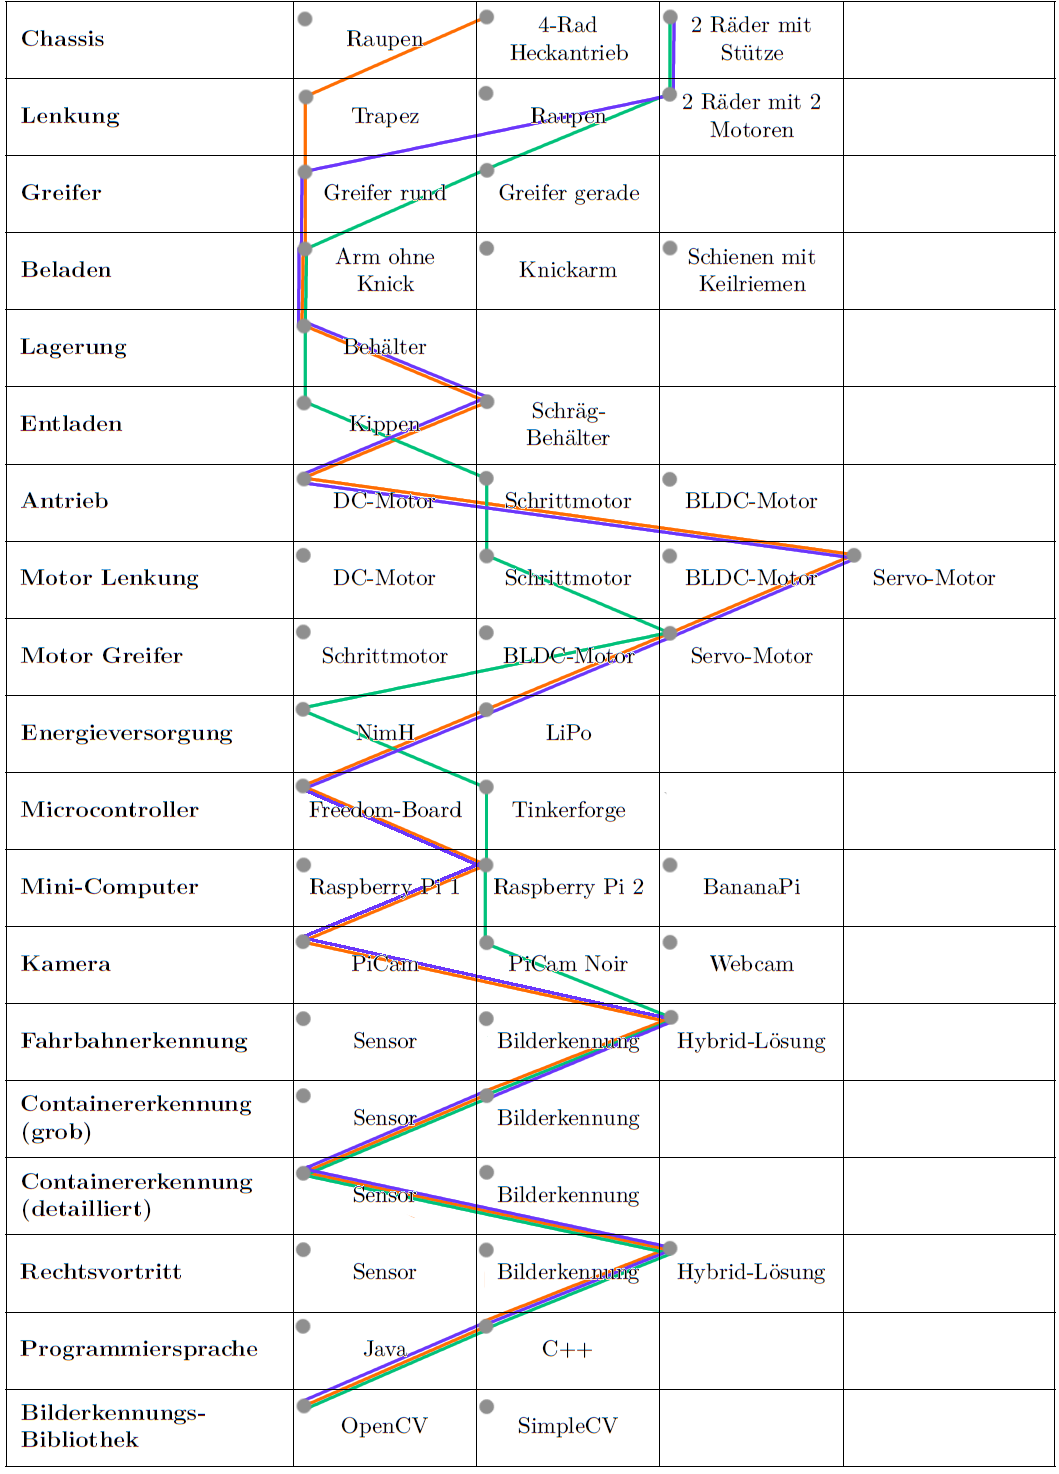
\includegraphics[width=1.0\textwidth]{fig/morphologischeKasten_mitKonzeptvarianten.png}
\caption{Morphologischer Kasten}
\label{fig:Morphologischer Kasten}
\end{figure}


\clearpage
% !TEX root = morphkasten.tex

\section{Chassis}


%############## RAUPEN
\subsection{Raupen}

\begin{figure} [hbp]
	\centering
	\begin{subfigure}[b]{0.4\textwidth}
		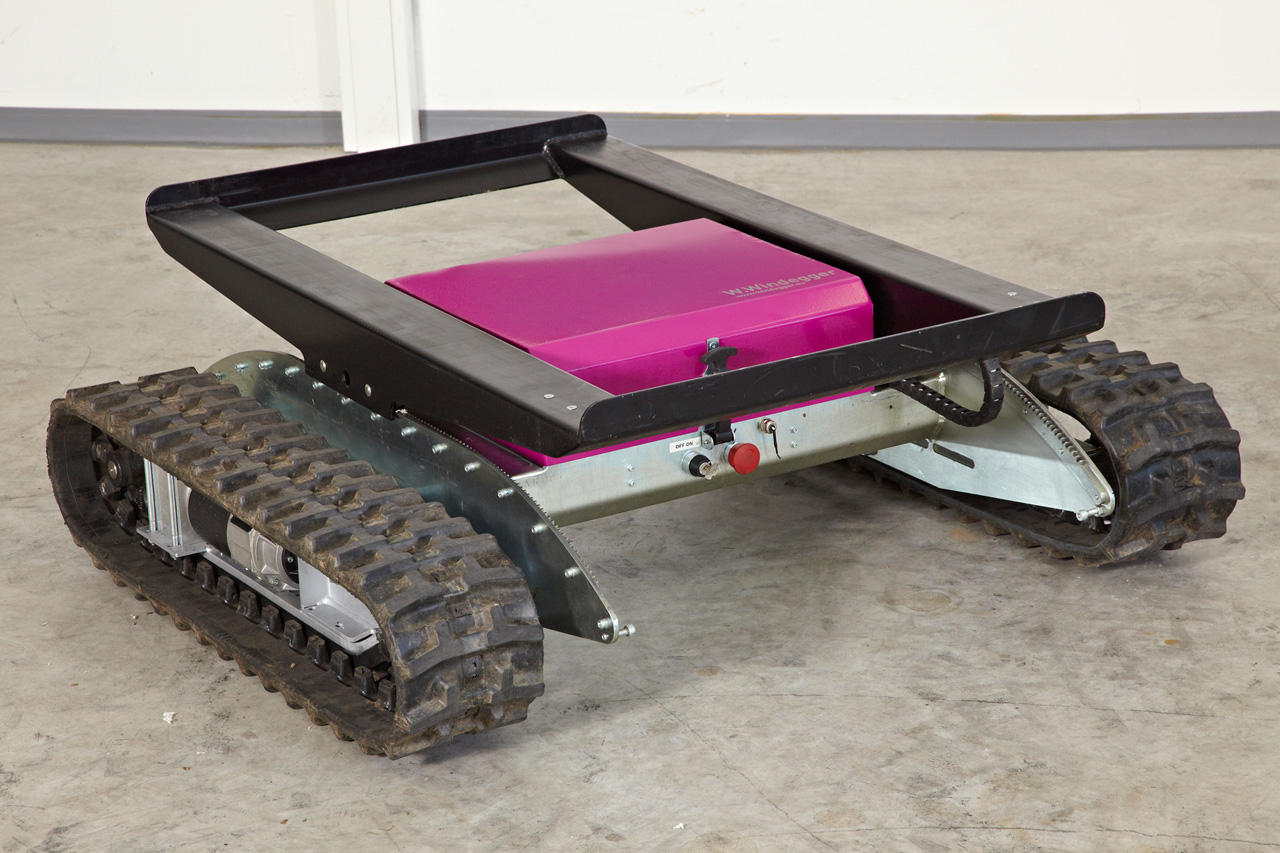
\includegraphics[width=\textwidth]{fig/Raupenfahrzeug.jpg}
		\caption{1. Situation: Modell 
		(Quelle: www.slowine-tech.de)}
	\end{subfigure}
	\hfill
	\begin{subfigure}[b]{0.36\textwidth}
		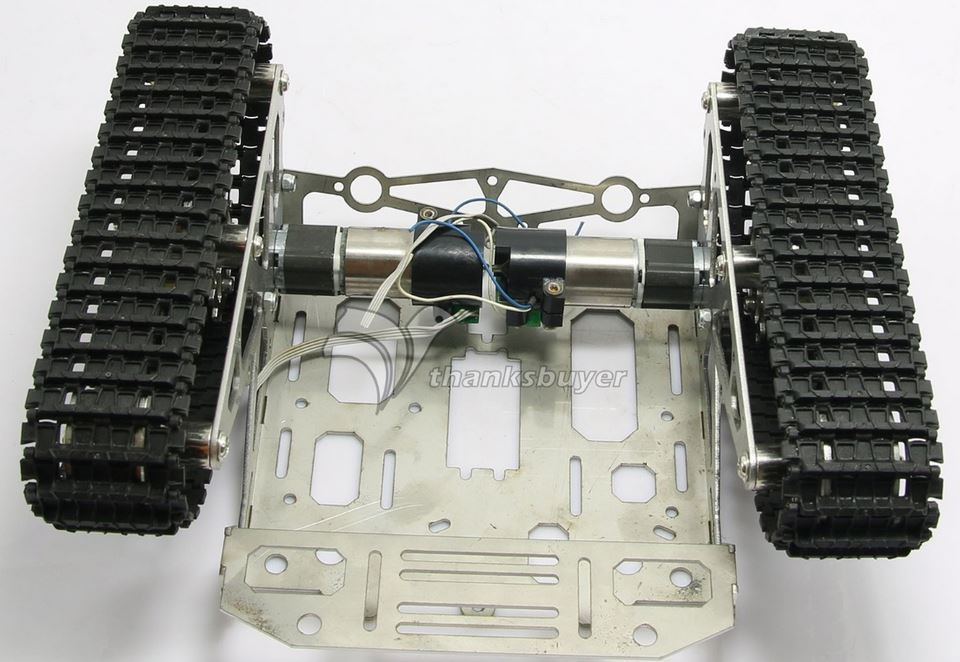
\includegraphics[width=\textwidth]{fig/Raupenfahrzeug-2.JPG}
		\caption{2. Situation: Ansicht von unten
		(Quelle: http://www.sainsmart.com/)}
\end{subfigure}
	\caption{Raupenfahrzeug}\label{fig:animals}
\end{figure}


\begin{table}[h]
\begin{tabular}{p{0.5\textwidth} | p{0.5\textwidth}}


 \textbf{Vorteile} & \textbf{Nachteile} \\ \hline
	 
\begin{itemize}
\item Lenkung sehr einfach realisierbar
\item Viele Beispiele im Internet verfügbar
\item Selbe Motoren für die Lenkung und den Antrieb
\end{itemize}

 
 &
 
\begin{itemize}
\item Schwerpunkt muss in der Mitte der Raupen sein
\item Längsämter als Räder
\item evtl. Schlupf zwischen Raupe und Antrieb
\item eher für Geländefahrten geeignet
\item gute Modellraupen sind teuer
\end{itemize}

\end{tabular}
\end{table}

\begin{table}[h]
\begin{tabular}{p{0.5\textwidth}p{0.5\textwidth}}


 \textbf{Risiken} & \\ \hline
	 
\begin{itemize}
\item Der Schwerpunkt, sollte für eine gute Lenkung, in der Mitte der Raupen und auf beide Raupen gleichmässig verteilt sein.
\end{itemize}
&
\begin{itemize}
\item Das finden von geeigneten Modellraupen mit unseren Abmassen könnte sich schwierig gestalten.
\end{itemize}


 
\end{tabular}
\end{table}

\pagebreak


%############## 4-Rad Heckantrieb
\subsection{4-Rad Heckantrieb}

\begin{figure} [hbp]
	\centering
	\begin{subfigure}[b]{0.45\textwidth}
		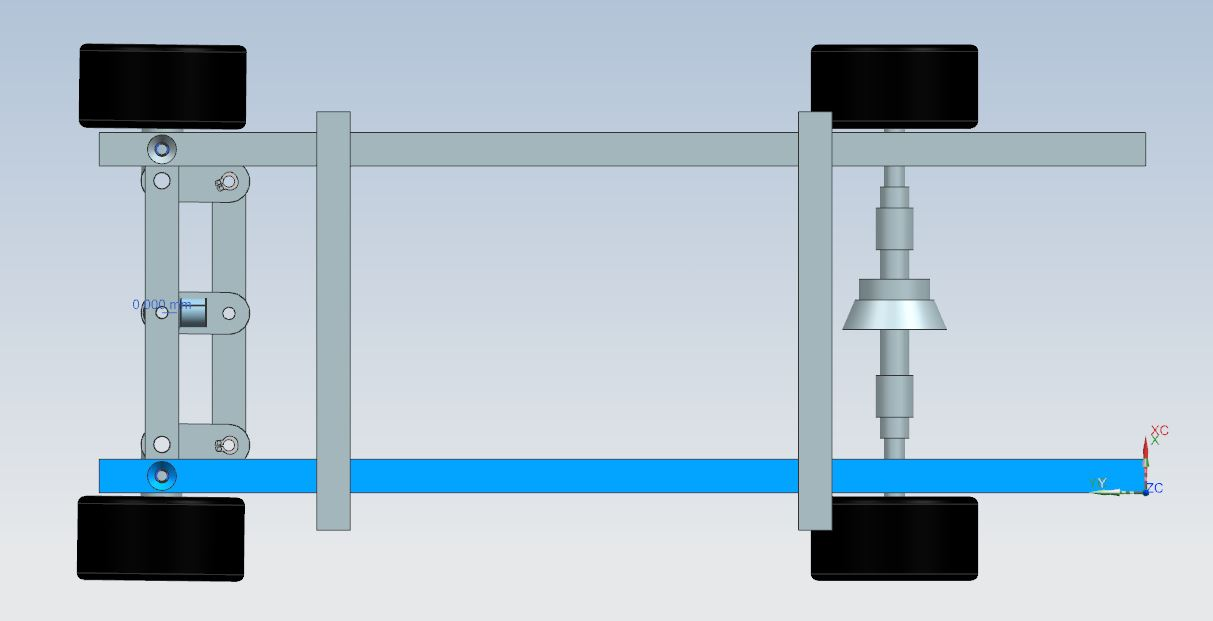
\includegraphics[width=\textwidth]{fig/4Rad-1.JPG}
		\caption{1. Situation: Ansicht von oben}
	\end{subfigure}
	\hfill
	\begin{subfigure}[b]{0.45\textwidth}
		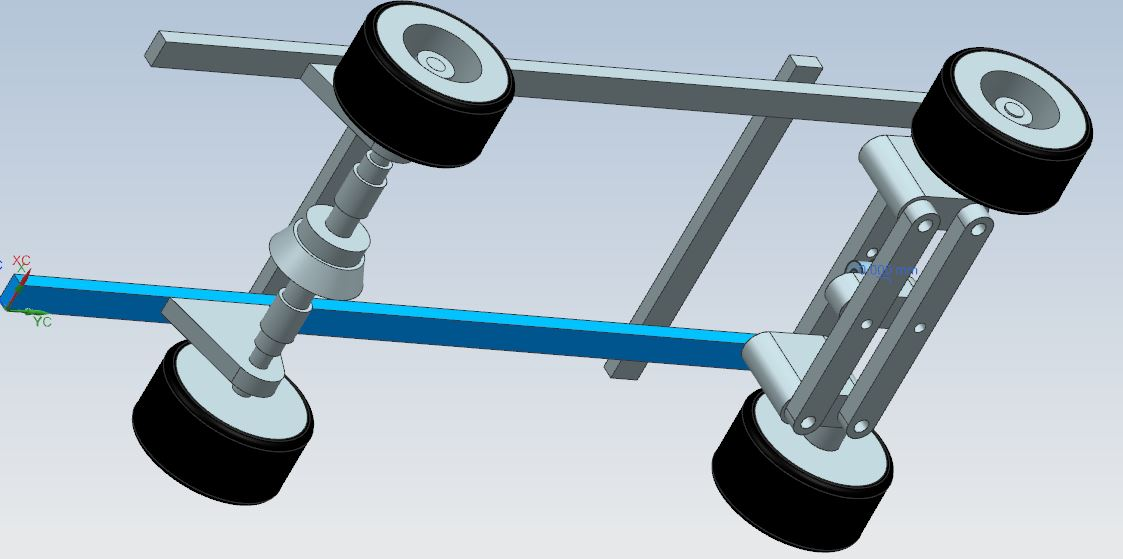
\includegraphics[width=\textwidth]{fig/4Rad-2.JPG}
		\caption{2. Situation: Ansicht von unten}
\end{subfigure}
	\caption{4-Rad mit Heckantrieb}\label{fig:animals}
\end{figure}

\begin{table}[h]
\begin{tabular}{p{0.5\textwidth} | p{0.5\textwidth}}


 \textbf{Vorteile} & \textbf{Nachteile} \\ \hline
	 
\begin{itemize}
\item Viel genutztes Prinzip im Modellbau
\item Viele Vorlagen im Internet
\item Klare Trennung zwischen Antrieb und Lenkung
\item Sehr Stabil
\end{itemize}

 
 &
 
\begin{itemize}
\item Für den Heckantrieb ist ein Differential notwendig
\item Es muss eine Lenkung eingebaut werden 
\item Regelung der Lenkung ist aufwendig
\end{itemize}

\end{tabular}
\end{table}

\begin{table}[h]
\begin{tabular}{p{0.5\textwidth}p{0.5\textwidth}}


 \textbf{Risiken} & \\ \hline
	 
\begin{itemize}
\item Ist das Fahrzeug zu lang, könnte man in der Kurve mit den Hinterrädern die Fahrbahn verlassen.
\end{itemize}
&
\begin{itemize}
\item Die Lenkung könnte zu unpräzise sein.
\end{itemize}

 
\end{tabular}
\end{table}

\pagebreak


%############## 3-Rad
\subsection{2-Rad mit Stützen}

\begin{figure} [hbp]
	\centering
	\begin{subfigure}[b]{0.4\textwidth}
		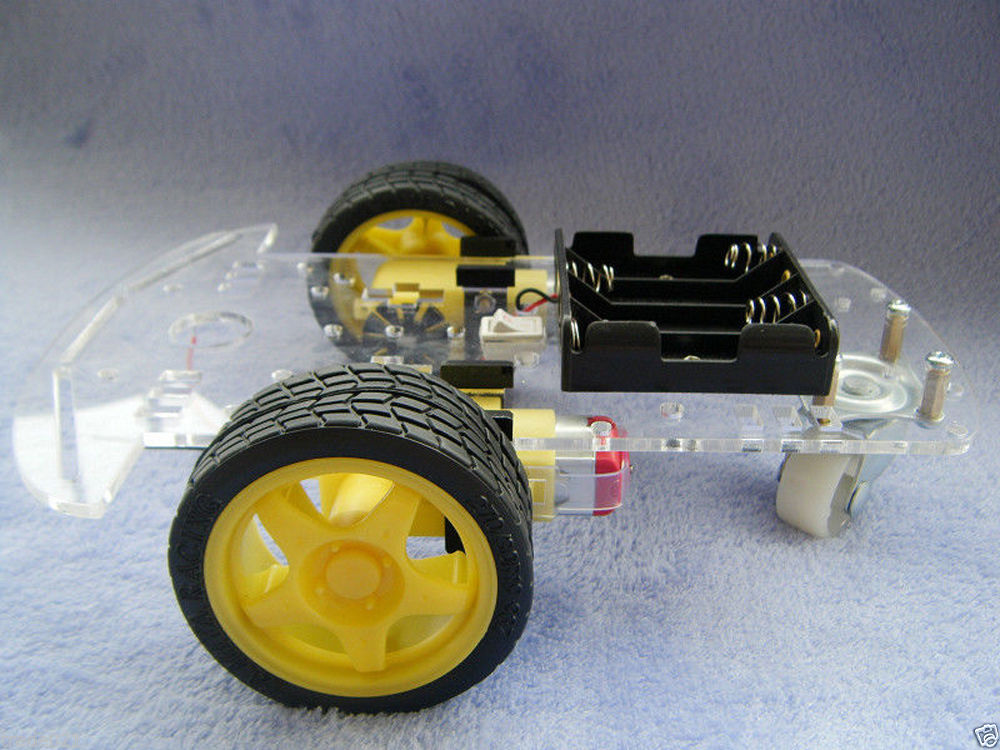
\includegraphics[width=\textwidth]{fig/3rad-1.jpg}
		\caption{1. Situation: Modell 
		(Quelle: www.sainsmart.com)}
	\end{subfigure}
	\hfill
	\begin{subfigure}[b]{0.36\textwidth}
		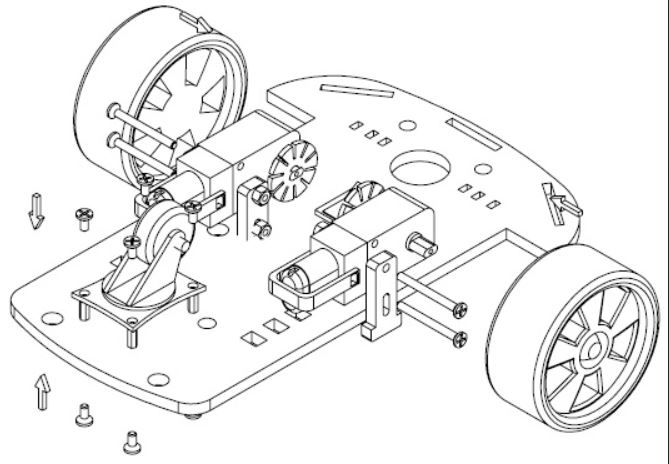
\includegraphics[width=\textwidth]{fig/3rad-3.JPG}
		\caption{2. Situation: Technische Zeichnung
		(Quelle: www.sainsmart.com)}
\end{subfigure}
	\caption{2-Rad Modell}\label{fig:animals}
\end{figure}

\begin{table}[h]
\begin{tabular}{p{0.5\textwidth} | p{0.5\textwidth}}


 \textbf{Vorteile} & \textbf{Nachteile} \\ \hline
	 
\begin{itemize}
\item Einfache Lenkung
\item Selber Motor für Antrieb und Lenkung
\item Sehr wendig
\item Konstruktiv einfach Realisierbar
\end{itemize}

 
 &
 
\begin{itemize}
\item Stabilität eher gering
\item Motoren müssen sehr genau sein
\item Grösse der Motoren für einen geeigneten Antrieb 
\end{itemize}

\end{tabular}
\end{table}

\begin{table}[h]
\begin{tabular}{p{0.5\textwidth}p{0.5\textwidth}}


 \textbf{Risiken} & \\ \hline
	 
\begin{itemize}
\item Bei einem 2-Rad Modell ist die Stabilität das grösste Problem. Beim Aufladen des Containers könnte das Fahrzeug kippen.
\end{itemize}
&
\begin{itemize}
\item Wenn die Antriebsräder in der Mitte montiert sind, braucht man vorne und hinten ein Stützrad oder eine Stützkugel. Diese könnten grössere Reibungskräfte verursachen.
\end{itemize}

 
\end{tabular}
\end{table}

\pagebreak

% !TEX root = ../Dokumentation.tex
\subsection{Lenkung}

\textbf{Funktionsbeschrieb}
\\[0.2cm]
Die Lenkung ist eine Achsschenkellenkung. Sie wird heute in fast allen PKWs, LKWs, Omnibussen und sonstige Nutzfahrzeugen eingesetzt. Bei dieser Art der Lenkung befinden sich die Räder auf einzeln lenkbaren Achsschenkeln, die jeweils mit einem Spurstangenhebel versehen sind. Die Spurstangenhebel sind ungefähr senkrecht zur Vorderachse bzw. ungefähr parallel zur Längsachse des Fahrzeugs ausgerichtet und mittels einer Spurstange miteinander verbunden. Dadurch werden beide Räder gleichzeitig gelenkt.\\[0.2cm]
\textbf{Komponentenbeschrieb}
\\[0.2cm]
Mit einem Servomotor wird über eine Kegelradverbindung der Lenkschubhebel angetrieben. Dieser treibt wiederum die Spurstange an, welche die Bewegung Über die Spurstangenhebel an die Räder weitergibt.
\begin{figure}[H]%Position festigen
\centering
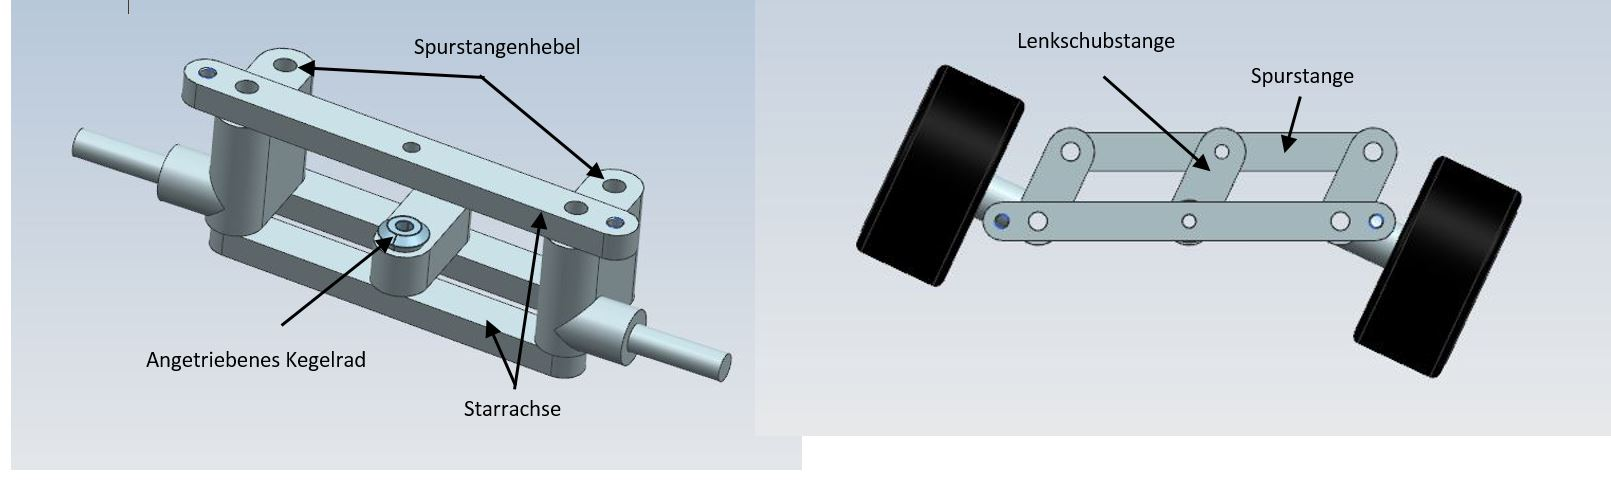
\includegraphics[width=1\textwidth]{03_Loesungskonzept/pictures/Achsschenkellenkung.JPG}
\caption{Konzept der Achsschenkellenkung}
\label{fig:activityRoute}
\end{figure}
\textbf{Begründung}\\[0.2cm]
Für die Bildverarbeitung ist das Lenken und konstante ausgleichen der Fahrbahn und Fahrtgeschwindigkeit mit zwei Motoren, welche jeweils ein Rad antreiben Nachteil. Darum ist das Lösungskonzept mit einer Achsschenkellenkung ausgestattet. Von der Konstruktiven seit ist die Achsschenkellenkung im Vergleich zwar aufwändiger aber für die Aufgabenstellung besser geeignet. Da dass Ziel ist einen möglichst konstanten Abstand zum Trottoir der Fahrbahn zu halten, ist die Regelung einer Achsschenkellenkung einfacher. Weitere Gründe, welche für die Achsschenkellenkung sprechen wurden schon im Kapitel \glqq{Chassis}\grqq  erläutert.
Die Begründung für die Wahl des Servomotors ist, dass die Lenkung keine 360° Bewegungen durchführen muss. Zudem ist die Drehzahl des Servos leicht zu steuern, ohne das zusätzlich eine Regelung eingebaut werden muss. 
\textbf{Berechnungen}\\[0.2cm]
Berechnung Drehmoment Servo Lenkung
Gewichtskraft auf jedes Rad Fg = m*g/4
Abstand l = 30mm
M = 2*Fg*l = 0.37Nm
Sicherheitsfaktor = 1.5 (da Beschleunigung- und Bremskräfte vernachlässigt werden)
M = 0.37*1.5 = 0.555Nm = 55.5Ncm\flushleft

% !TEX root = morphkasten.tex

\section{Greifer}


%##############
\subsection{Greifer rund}
\begin{figure} [hbp]
	\centering
	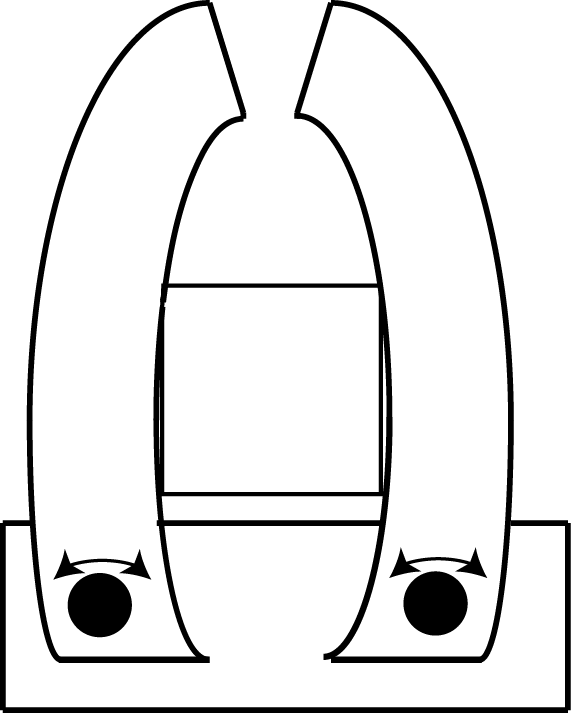
\includegraphics[width=0.5\textwidth]{fig/Greifer_rund.png}
	\caption{runder Greifer}
\end{figure}


\begin{table}[h]
\begin{tabular}{p{0.5\textwidth} | p{0.5\textwidth}}


 \textbf{Vorteile} & \textbf{Nachteile} \\ \hline
	 
\begin{itemize}
\item 2 Auflagepunkte am Container
\item Mit Zahnradübersetzung ist das Schliessen/Öffnen mit einem Motor möglich
\item keine Sensoren nötig um Schliessvorgang zu bestätigen
\item Automatische Zentrierung
\end{itemize}

 
 &
 
\begin{itemize}
\item Auf beiden Seiten hohe bzw. 2 Greiferbacken nötig um Stabilität zu garantieren
\item wenig Platz um Motor zu befestigen
\end{itemize}

\end{tabular}
\end{table}

\begin{table}[h]
\begin{tabular}{p{0.5\textwidth}p{0.5\textwidth}}


 \textbf{Risiken} & \\ \hline
	 
\begin{itemize}
\item Breitenbegrenzung überschreiten wegen der Länge des Greifers
\end{itemize}

 
\end{tabular}
\end{table}

\pagebreak


%##############
\subsection{Greifer gerade}
\begin{figure} [hbp]
	\centering
	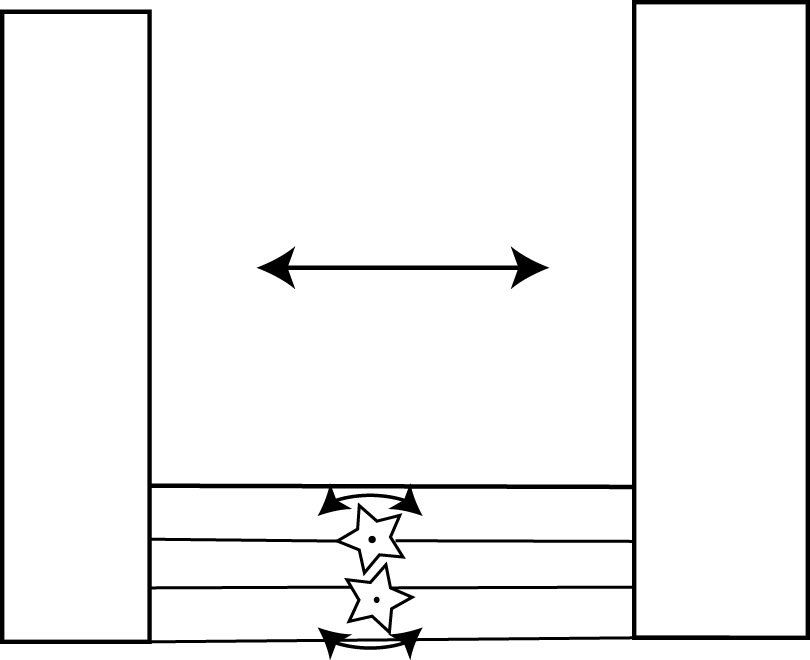
\includegraphics[width=0.5\textwidth]{fig/Greifer_gerade.png}
	\caption{gerader Greifer}
\end{figure}

\begin{table}[h]
\begin{tabular}{p{0.5\textwidth} | p{0.5\textwidth}}


 \textbf{Vorteile} & \textbf{Nachteile} \\ \hline
	 
\begin{itemize}
\item grosse Auflagefläche für Container
\item Mit Zahnradübersetzung nur ein Motor zum Schliessen/Öffnen nötig
\end{itemize}

 
 &
 
\begin{itemize}
\item sehr breiter Greifer bei unpräziser Positionierung nötig
\item aufwändige Führung
\item hohes Gewicht
\item wenig Platz für Motor
\end{itemize}

\end{tabular}
\end{table}

\begin{table}[h]
\begin{tabular}{p{0.5\textwidth}p{0.5\textwidth}}


 \textbf{Risiken} & \\ \hline
	 
\begin{itemize}
\item Stabilität des Greifer fraglich
\item Motorenüberlastung
\end{itemize}

 
\end{tabular}
\end{table}

\pagebreak

% !TEX root = ../Dokumentation.tex
\subsection{Beladen und Greifer}

\textbf{Funktionsbeschrieb}
\begin{figure}[H]
\centering
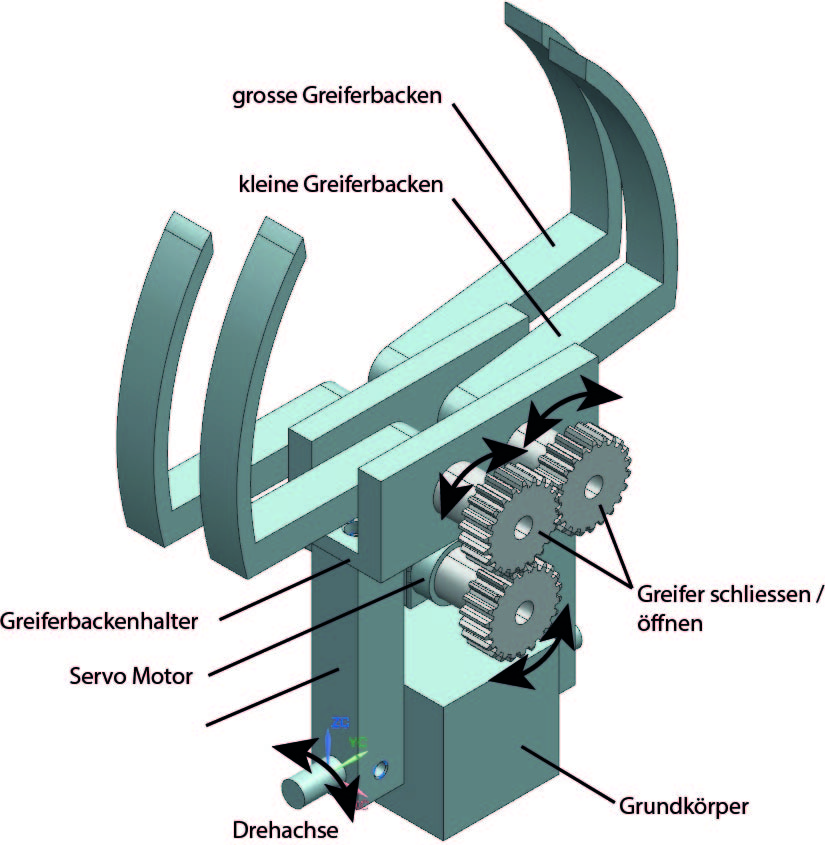
\includegraphics[width=0.5\textwidth]{03_Loesungskonzept/pictures/greifer3.jpg}
\caption{Greifer}
\end{figure}\flushleft

Der Greifer ist auf der Grundplatte des Fahrzeuges montiert. Im Grundkörper wird die Welle für die Drehung des Greifers montiert. Die Welle wird von einem Servo Motor angetrieben. Um gute Laufeigenschaften zu erreichen werden Lagerbüchsen eingebaut. Auf der Drehachse sind die beiden Seitenplatten des Greifers montiert. Auf den Seitenplatten wird der Greifbackenhalter verschraubt.  Der Servo Motor für die Funktion Greifer schliessen/ öffnen wird am Greifbackenhalter befestigt. Auf dem Servo wird ein Zahnrad montiert, das über die gleichen Zahnräder die Greiferbacken öffnet bzw. schliesst. Die Greiferbacken sind so konzipiert, dass die 2 längeren und 2 kürzeren an verschiedenen Flächen greifen. Damit wird erreicht, dass der Container stabil bleibt während des ganzen Einladeprozesses. 

\begin{figure}[H]
\centering
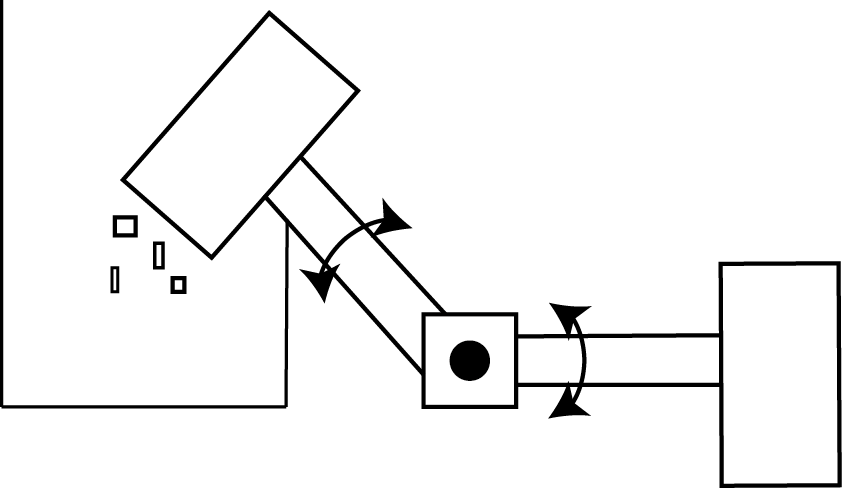
\includegraphics[width=0.5\textwidth]{03_Loesungskonzept/pictures/Beladen_1.png}
\caption{Einladeprozess}
\end{figure}\flushleft
Der Greifer ist während des Fahren in oberer Position gelagert, damit die Abmasse der Aufgabenstellung eingehalten werden können. Der Greifer wird erst auf horizontale Richtung bewegt, nachdem der Wagen still steht und richtig positioniert ist.
Die rechte Fahrzeugkante wird auf 25mm +/- 5mm zum Trottoirrand positioniert. In Fahrtrichtung beträgt die maximale zulässige Positionierungsgenauigkeit +/- 10mm.

\begin{figure}[H]
\centering
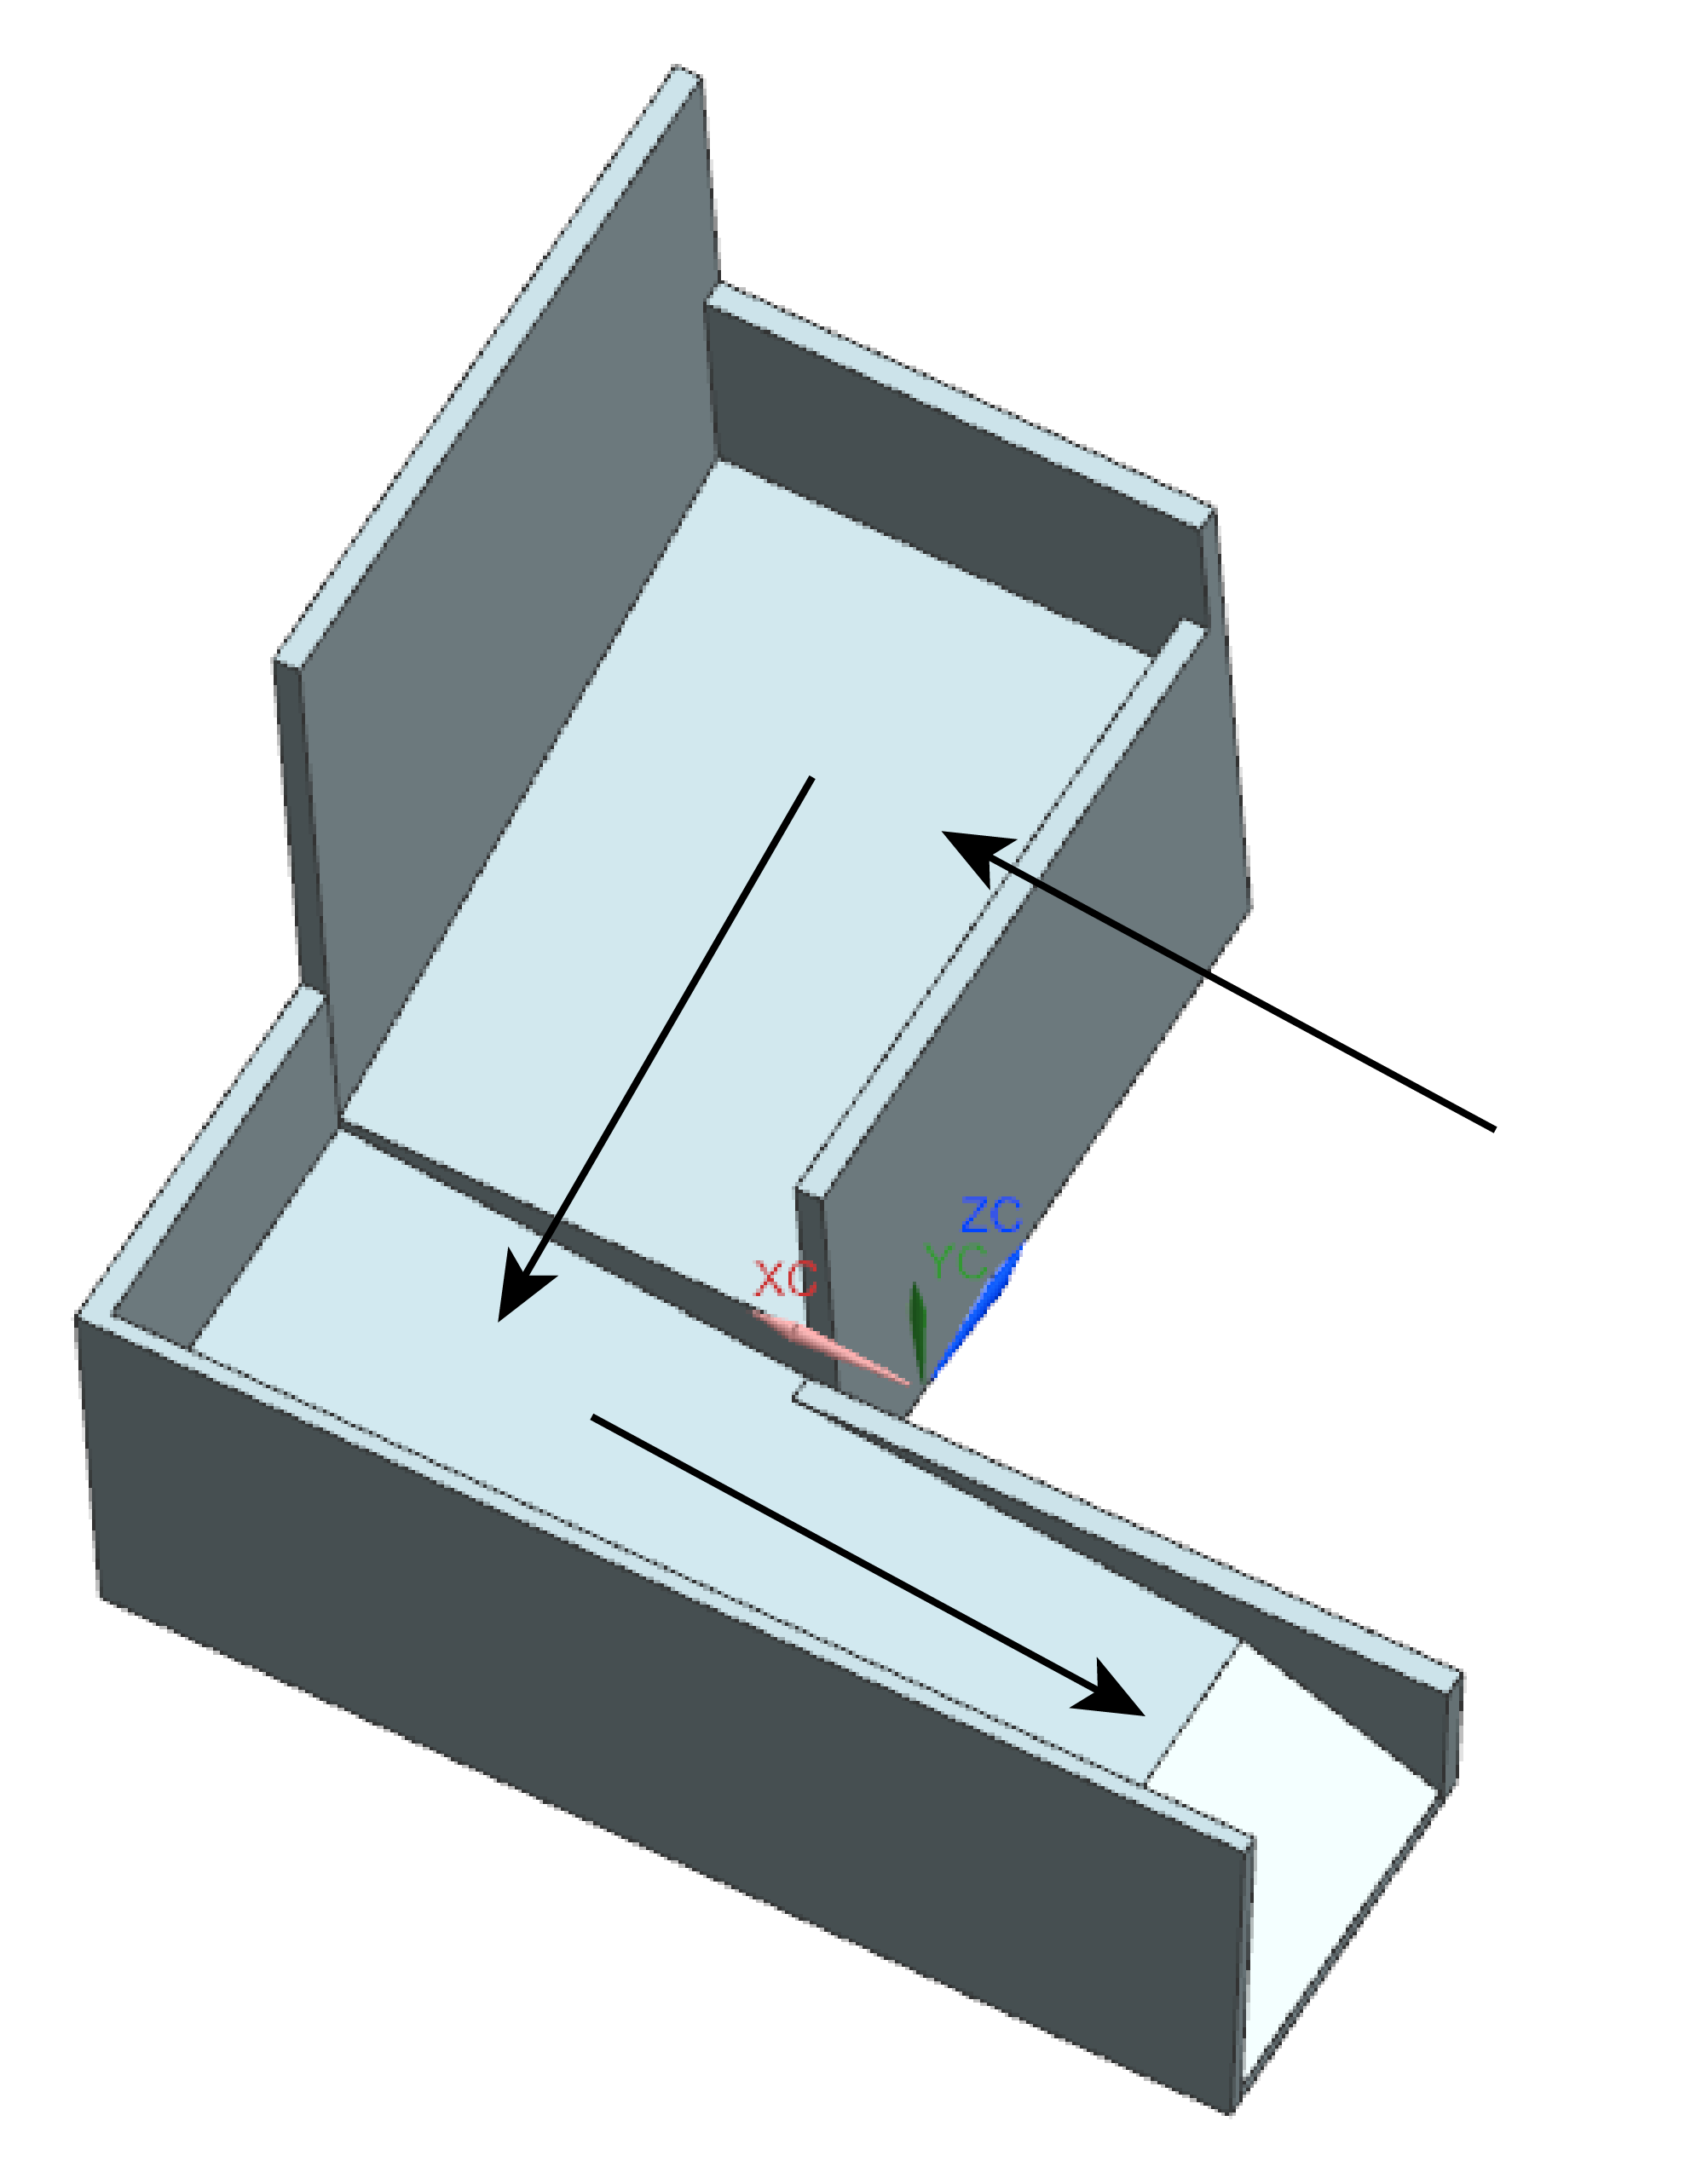
\includegraphics[width=0.5\textwidth]{03_Loesungskonzept/pictures/behaelter.png}
\caption{Schüttgutfluss in den beiden Behältern}
\end{figure}\flushleft
Der Container wird in den ersten Behälter entleert. Durch den schrägen Boden rutscht das Schüttgut in den zweiten Behälter. Am Ende des zweiten Behälters wird ein Klappe montiert, damit die Schrauben und Mutter nicht herausfallen. Die Klappe wird durch einen Servo Motor gehalten und erst am Schluss beim Entladebehälter geöffnet.\\[0.2cm]

\textbf{Komponentenbeschrieb}\\[0.2cm]
\begin{itemize}
\item Zahnräder aus Kunststoff, Durchmesser = 15 (Einkaufteil)
\item Greiferbacken aus Kunststoff (Druckteil)
\item Grundkörper, Seitenplatte, Greifbackenhalter und Wellen werden aus Aluminium gefertigt.
\item Behälter aus Acrylglas 3mm Dicke (Laserzuschnitt)
\item Technische Daten des Motors Greifer:
\begin{itemize}
\item Stellzeit bei 4.8 Volt: 0.1 sec (50°) 
\item Stellzeit bei 6 Volt: 0.08 sec (50°) 
\item Betriebsspannung: 4.6/6 V
\item Stell-Moment bei 4.8 Volt: 18 Ncm
\item Stell-Moment bei 6 Volt: 20 Ncm 
\end{itemize}
\end{itemize}
\textbf{Berechnungen}\\[0.2cm]
Servo Motor für Greifer schliessen /
Berechnung des benötigten Drehmoments: 
\begin{itemize}
\item Haftreibung auf 0.7 geschätzt
\item Masse Container $m = 0.075kg$
\item Gewichtskraft = $m\cdot g = 0.74 N$
\item Kraft $F = \frac{0.5\cdot 0.74}{0.7} = 0.53 N$
\item Abstand $l = 80mm$ (Drehpunkt zu Greiffläche)
\item $M = F\cdot l = 0.04 Nm = 4 Ncm$
\item Sicherheitsfaktor = 2
\item M = $4\cdot 2 = 8 Ncm$
\end{itemize}
Servo Motor für Greifarm drehen:
\begin{itemize}
\item Gewichtskraft Container $Fc = 0.075kg\cdot 9.81 = 0.74 N$
\item Gewichtskraft Greifarm: $Fgr = 0.3kg\cdot 9.81 = 2.94 N$
\item Benötigtes Moment:
$M = Fgr\cdot 0.05m+Fc\cdot 0.1m = 0.147Nm+0.07Nm = 0.217Nm = 21.7Ncm$
\item Sicherheitsfaktor = 2 wegen Abschätzug des Greifergewichts und vernachlässigter Trägheitskräfte
\item $M = 2 \cdot 21.7 = 43.4 Ncm$
\end{itemize}

% !TEX root = morphkasten.tex

\section{Lagerung}


%##############
\subsection{Behälter}

Grafik

\begin{table}[h]
\begin{tabular}{p{0.5\textwidth} | p{0.5\textwidth}}


 \textbf{Vorteile} & \textbf{Nachteile} \\ \hline
	 
\begin{itemize}
\item Vorteil 1
\item Vorteil 2
\item Vorteil 3
\item ...
\end{itemize}

 
 &
 
\begin{itemize}
\item Nachteil 1
\item Nachteil 2
\item Nachteil 3
\item ...
\end{itemize}

\end{tabular}
\end{table}

\begin{table}[h]
\begin{tabular}{p{0.5\textwidth}p{0.5\textwidth}}


 \textbf{Risiken} & \\ \hline
	 
\begin{itemize}
\item Risiko 1
\item Risiko 2
\end{itemize}
&
\begin{itemize}
\item Risiko 3
\item ...
\end{itemize}

 
\end{tabular}
\end{table}

\pagebreak


% !TEX root = ../Dokumentation.tex
\subsection{Entladen}

\textbf{Funktionsbeschrieb}\\[0.2cm]
\begin{figure}[H]
\centering
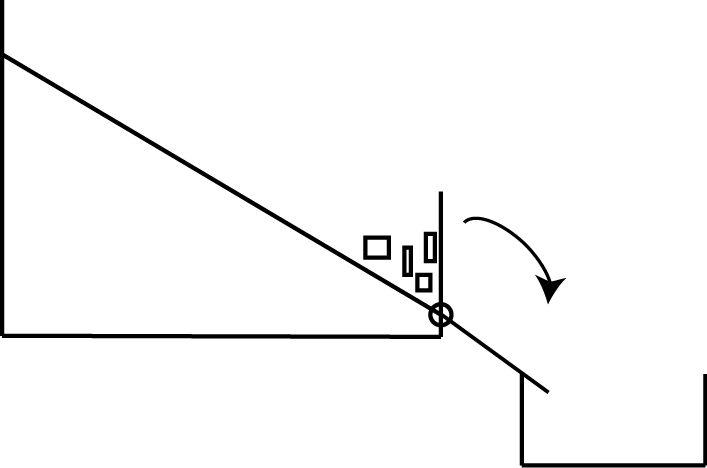
\includegraphics[width=0.5\textwidth]{03_Loesungskonzept/pictures/Entladen_Schraegbehaelter.png}
\caption{Entladen}
\end{figure}

\ Beim Entladevorgang fährt das Fahrzeug bis auf 20mm +/- 5mm an den Rand des Entsorgungsbecken. Anschliessend wird die Klappe gelöst und diese fällt auf den Rand des Entsorgungsbecken. Über die Klappe rutscht das Schüttgut in das Entsorgungsbecken. Nach erfolgter Abladung fährt das Fahrzeug kurz nach links, damit das ganze Fahrzeug im Zielbereich steht. Dabei hängt die Klappe nach unten.

\textbf{Komponentenbeschrieb}

\ Die Klappe besteht aus einem handelsüblichen Scharnier auf dem eine Platte aus Acrylglas befestigt ist.
Die Klappe wird durch einen Servomotor gehalten.\\
Technische Daten des Servomotors:
\begin{itemize}
\item Stellzeit bei 4.8 Volt: 0.1 sec (50°) 
\item Stellzeit bei 6 Volt: 0.08 sec (50°) 
\item Betriebsspannung: 4.6/6 V
\item Stell-Moment bei 4.8 Volt: 18 Ncm
 \item Stell-Moment bei 6 Volt: 20 Ncm 
\end{itemize}

\textbf{Berechnungen}
\ Die Berechnungen zum Servo Motor für die Klappe sind schon im Kapitel Beladen zu finden.

% !TEX root = ../Dokumentation.tex
\subsection{Antrieb}

\textbf{Funktionsbeschrieb}\\[0.2cm]
Als Antrieb wird ein DC-Getriebemotor verwendet, der an der Unterseite montiert wird und für die Vor- sowie Rückwärtsbewegungen des Fahrzeugs zuständig ist.
Die aktuelle Drehzahl des Motors wird von einem Encoder erfasst. Dieser wiederum sendet die gemessenen Daten an den Microcontroller der schlussendlich die Anzahl Umdrehungen reguliert.\\[0.2cm]
\textbf{Komponentenbeschrieb}
\begin{figure}[H]
\centering
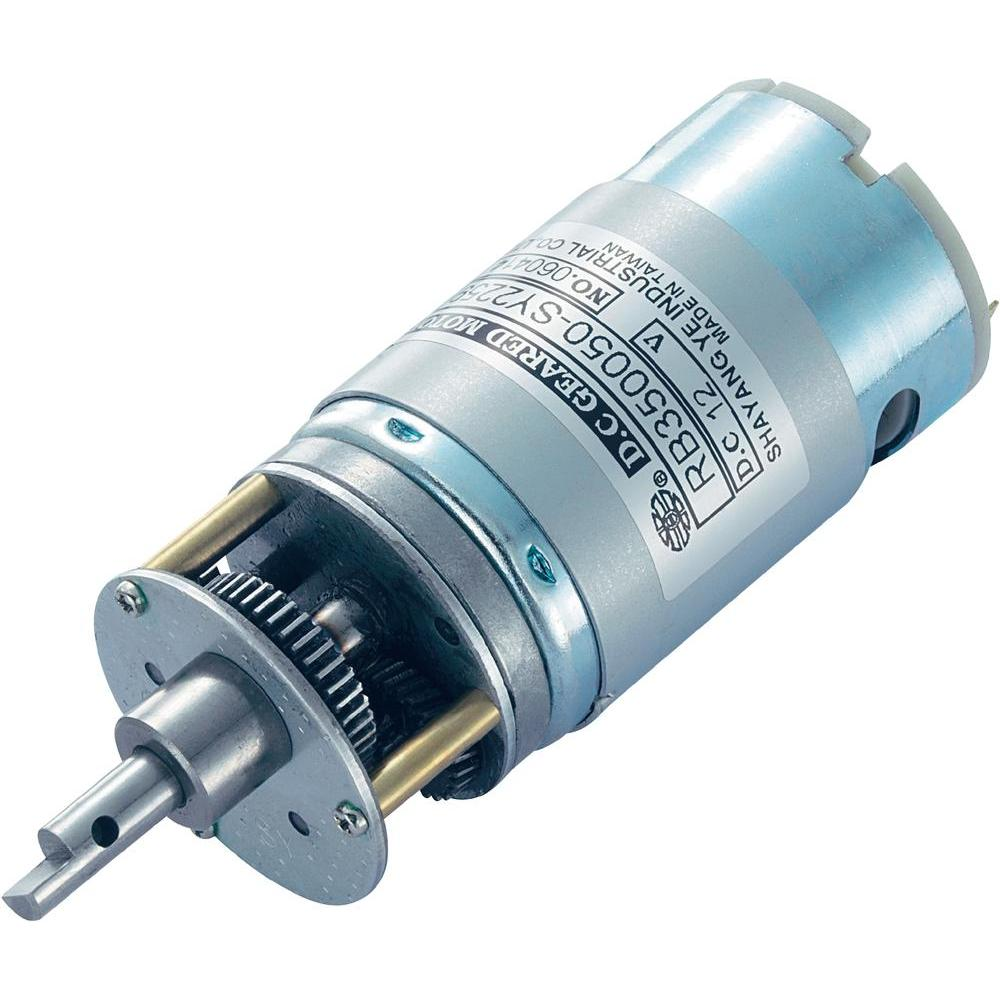
\includegraphics[width=0.5\textwidth]{03_Loesungskonzept/pictures/antrieb.jpg}
\caption{Antrieb  (Quelle:http://www.conrad.ch)}	
\end{figure}\flushleft
Als voraussichtlicher Favorit wurde ein Hochleistungsgetriebemotor von Modelcraft ausgewählt. Die technischen Daten sind folgende:
\begin{itemize}
\item Leerlaufstrom: 0.32 A
\item Last-Drehzahl: 317 U/min
\item Leerlauf-Drehzahl: 333 U/min
\item Betriebsspannung: 12 V DC
\item Spitzendrehmoment: 2.23 Nm
\item Max. Laststrom: 0.7 A
\end{itemize}
\textbf{Begründung}\\[0.2cm]
Der ausgewählte Motor punktet vor allem aufgrund seiner kleinen und kompakten Bauform. Da der Montageort für den Antrieb am Fahrzeug nicht verändert werden kann, ohne umständliche Wellen zu installieren, ist die Baugrösse relativ beschränkt.
Ein weiterer Punkt ist, dass er sich als Gleichstrommotor leicht ansteuern lässt und damit die Handhabung vereinfacht.
Zudem zeichnet er sich mit einer hohen Drehzahl und grossem Drehmoment aus und ist dennoch verhältnismässig günstig in der Anschaffung.


% !TEX root = morphkasten.tex

\section{Motor Lenkung}


%##############
\subsection{DC-Motor}

Im Kapitel 7.1 wurde die Variante DC-Motor bereits beschrieben.


%##############
\subsection{Schrittmotor}
Im Kapitel 7.2 wurde die Variante Schrittmotor bereits beschrieben.

%##############
\subsection{BLCD-Motor}
Im Kapitel 7.3 wurde die Variante BLCD-Motor bereits beschrieben.

%##############
\subsection{Servo-Motor}

\begin{figure}[h!]%Position festigen
\centering
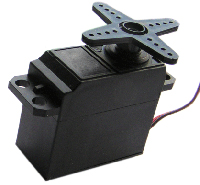
\includegraphics[width=0.5\textwidth]{fig/servo.jpg}
\caption{Servo-Motor (Quelle: http://www.sachsendreier.com/asw/clernen/servo/servo.html)}
\label{fig:Java}
\end{figure}

\begin{table}[h]
\begin{tabular}{p{0.5\textwidth} | p{0.5\textwidth}}


 \textbf{Vorteile} & \textbf{Nachteile} \\ \hline
	 
\begin{itemize}
\item Sehr präzise
\item Sehr hoher Wirkungsgrad
\end{itemize}

 
 &
 
\begin{itemize}
\item Komplexe Ansteuerung
\item Hoher Anschaffungspreis
\item Hat einen begrenzten Drehwinkel
\item Relativ empfindlich
\end{itemize}

\end{tabular}
\end{table}

\begin{table}[h]
\begin{tabular}{p{0.5\textwidth}p{0.5\textwidth}}


 \textbf{Risiken} & \\ \hline
	 
\begin{itemize}
\item Erhötes Risiko, dass der Motor bei Versuchen Schaden nimmt.
\end{itemize}

 
\end{tabular}
\end{table}

\pagebreak

% !TEX root = morphkasten.tex

\section{Motor Greifer}


%##############
\subsection{Schrittmotor}
Im Kapitel 7.2 wurde die Variante Schrittmotor bereits beschrieben.

%##############
\subsection{BLCD-Motor}
Im Kapitel 7.3 wurde die Variante BLCD-Motor bereits beschrieben.

%##############
\subsection{Servo-Motor}
Im Kapitel 8.4 wurde die Variante Servo-Motor bereits beschrieben.
\pagebreak

% !TEX root = ../Dokumentation.tex
\subsection{Energieversorgung}
%
\textbf{Funktionsbeschrieb}\\[0.2cm]
Das autonome Entsorgungsfahrzeug muss mit Energie versorgt werden. Dazu werden Akkumulatoren eingesetzt, welche das Gerät während dem gesamten Einsatz mit Strom versorgen. 
\\[0.2cm]
\textbf{Komponentenbeschrieb}\\[0.2cm]
Um die Energieversorgung zu gewährleisten, werden zwei Lithium-Polymer-Akkumulatoren mit einer Spannung von 11.1 und 7.4 Volt verwendet.
Der 11.1-Volt Akkumulator gewährleistet die Versorgung der Motoren und weist eine Kapazität von 2400 mAh auf. Für die empfindlicheren Systeme ist der 7.4 Volt LiPo zuständig, der eine Kapazität von 500mAh besitzt.
Die Kapazitäten beziehen sich auf die Resultate der Berechnungen, welche im Verlauf des Kapitels noch beschrieben werden.
\begin{figure}[H]
\centering
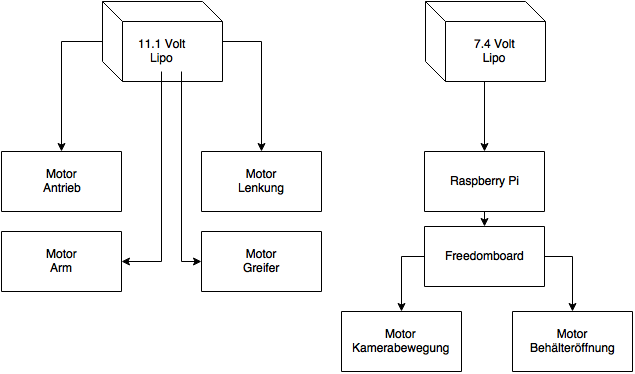
\includegraphics[width=0.8\textwidth]{03_Loesungskonzept/pictures/speisung.png}
\caption{Aufteilung der Akkumulatoren}	
\end{figure}
\textbf{Begründung}\\[0.2cm]
Die Entscheidung wird damit begründet, dass Lithium-Polymer-Akkumulatoren in einem vielfältigen Sortiment erhältlich sind und damit eine grosse Flexibilität bei der Auswahl ermöglichen. Somit würde sich auch die Suche nach einem Ersatz bei allfälligen Änderungen vereinfachen. Ausserdem weisen LiPos, im Vergleich zu anderen Akkumulatoren, eine wesentlich kompaktere Bauform auf, was entscheidend für die Auswahl war. \\[0.2cm]
\textbf{Berechnungen}\\[0.2cm]
Leistungsberechnungen:
\begin{itemize}
\item Servomotor für die Lenkung:
\[
P=2\cdot \pi\cdot N\cdot M \to 2\cdot \pi\cdot 0.92\frac{U}{sec}\cdot 0.65Nm = 3.76W
\]
\item Servomotoren für Kamerabewegung und Greifer:
\[
P=2\cdot \pi\cdot N\cdot M \to 2\cdot \pi\cdot 0.72\frac{U}{sec}\cdot 0.18Nm = 0.81W
\]
\item Servomotor für den Greiferarm:
\[
P=2\cdot \pi\cdot N\cdot M \to 2\cdot \pi\cdot 1.14\frac{U}{sec}\cdot 0.32Nm = 2.5W
\]
\item DC-Motor für den Antrieb:
\[
P=2\cdot \pi\cdot N\cdot M \to 2\cdot \pi\cdot 5.258\frac{U}{sec}\cdot 2.23Nm = 73.98W
\]
\item DC-Motor für die Behälteröffnung:
\[
P=2\cdot \pi\cdot N\cdot M \to 2\cdot \pi\cdot 16.6\frac{U}{sec}\cdot 0.028Nm = 2.9W
\]
\end{itemize}
\newpage
Kapazitätenberechnungen:
\begin{itemize}
\item DC-Motor für den Antrieb:
\[
\frac{P\cdot t}{U} \to \frac{73.98W\cdot0.25h}{12V}= 1.54 Ah
\]
\item DC-Motor für die Behälteröffnung:
\[
\frac{P\cdot t}{U} \to \frac{2.9W\cdot0.25h}{4.8V}= 0.15 Ah
\]
\item Servomotor für die Lenkung:
\[
\frac{P\cdot t}{U} \to \frac{3.76W\cdot0.25h}{4.8V}= 0.19 Ah
\]
\item Servomotor für den Greiferarm:
\[
\frac{P\cdot t}{U} \to \frac{2.5W\cdot0.25h}{4.8V}= 0.13 Ah
\]
\item Servomotoren für Kamerabewegung und Greifer:
\[
\frac{P\cdot t}{U} \to \frac{0.81W\cdot0.25h}{4.8V}= 0.04 Ah
\]
\item Mini-Computer:
\[
I\cdot t \to 2A*0.25h = 0.5 Ah
\]
\item Benötigte Kapazität für den 11.1 Volt Akkumulator:
\[
1.54Ah+0.15Ah+0.19Ah+0.13Ah+0.04Ah = 2.05Ah
\]
\item Benötigte Kapazität für den 7.4 Volt Akkumulator:
\[
0.5Ah
\]
\end{itemize}
\subsubsection{Akkuüberwachung Schwellwertberechnung}
Damit die LiPo-Akkumulatoren nicht zerstört werden, muss sichergestellt werden das diese nicht tief entladen werden. Dies wird über das Freedomboard gelöst. Die Akkuspannung wird über einen Analog - Digitalwandler eingelesen. Wenn die Akkuspannung einen gewissen Wert unterschreiten, werden die Verbraucher an den Akkus "abgeschaltet". Eine Lipozelle sollte die Zellenspannung von 3.7V nicht unterschreiten. Im Normalfall sollten alle Zellen einzeln überwacht werden, dies ist jedoch im Rahmen dieses Prototypen nicht angemessen. Als Kompromiss wird gesamte Ausgangsspannung gemessen. Das heisst zwei beziehungsweise drei Zellen in Serie (je nach Akku).\\
Das Freedomboard kann nur Spannungen bis 3.3V einlesen. Daher ist ein Spannungsteiler nötig. Damit dieser Wert sicher nicht überschritten wird, wird mit einer maximal zulässigen Spannung von 3V gerechnet. Für UAkku wurde 13V gewählt, damit der AD-Wandler sicher nie 3V erreicht.\\
Für den 11.1V Akku:
\[	U_Akku/U_Frd=R1/R2\]
\[	13V/3V=4.33=g\]
Gewählt:
\[	R2=10k R1=R2*4.33=43kOhm\]
Der Abschaltwert des drei Zellen Akkus ist 3.7V * 3 = 11.1V.
Nach dem Spannungswandler entspricht dies einer Spannung von \[Uin/g=11.1V*10kOhm/(10kOhm+43kOhm)=2.075V\]
3.3V enspricht 65'535. Somit entspricht eine Spannung von 2.075V einem eingelesenen Spannungswert von 41592. Falls dieser Wert über längere (wenige Sekunden) unterschritten wird, wird eine Nachricht an das Raspberry gesendet und das System heruntergefahren.

Für den 7.1V (logik) Akku wurde mit einer maximale Spannung von 8.5V gerechnet:
\[	U_Akku/U_Frd=R1/R2\]
\[	8.5V/3V=2.83\]
Gewählt:
\[	R2=10k R1=R2*2.83=28.3kOhm\]
Für UAkku wurde 7.4V als Abschaltwert gewählt.\\
7.4V nach dem Spannungswandler entspricht einer Spannung von \[Uin/g=7.4V*10kOhm/(10kOhm + 28.3kOhm)=1.947\]
3.3V enspricht 65'535. Somit entspricht eine Spannung von 1.974V einem eingelesenen Spannungswert von 38673. Dieser Wert musste angepasst werden, da der Akku zu früh abschaltete, da unter Last die Akkuspannung kurzzeitig sinkt. Ausgehend von dem gemessenen Wert von 32158 und einer Akkuspannung von 7.55V wurde der neue Wert von 31513 berechnet.
\\[0.2cm]
\textbf{Vergleich Konzept und Umsetzung}\\[0.2cm]
Die Akkuüberwachung konnte einfacher realisiert werden, als es im Pren1 konzipiert war. Dies deshalb, weil bei der Energieversorung auf eine galvanische Trennung der beiden Akkumulatoren verzichtet wurde. Dies ermöglichte das direkte einlesen des Spannungswertes über einen Spannungsteiler. Geplant war ursprünglich eine Vergleicherschaltung mit einem Operationsverstärker für den 11.1V Akkumulator. Diese Vereinfachung war auch sicher ein Grund auf die galvanische Trennung zu verzichten.


% !TEX root = morphkasten.tex

\section{Microcontroller}


%##############
\subsection{Freedom-Board}
\begin{figure}[h]
	\centering
	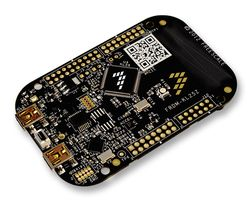
\includegraphics[width=0.5\textwidth]{fig/freedomboard.png}
	\caption{Freedomboard KL25 von Freescale (Quelle:http://ch.farnell.com/)}
	%http://ch.farnell.com/productimages/standard/de_DE/freescalesemiconductor-frdm-kl25z-40.jpg
\end{figure}


\begin{table}[h]
\begin{tabular}{p{0.5\textwidth} | p{0.5\textwidth}}


 \textbf{Vorteile} & \textbf{Nachteile} \\ \hline
	 
\begin{itemize}
\item Im Preisrahmen, ein Board gibt es ab 20Fr.-
\item Wurde an der Hochschule bereits eingesetzt(mögliche Ansprechpersonen)
\item Vereinfachte Programmierung mit Processor Expert
\item Kann zu Testzwecken ausgeliehen werden
\end{itemize}

 &
 
\begin{itemize}
\item Besitzt ein Betriebssystem $\Rightarrow$ weniger Hardware nahe
\item Keine zusätzlichen Module (weitere Hardware muss angebunden werden)
\end{itemize}

\end{tabular}
\end{table}

\begin{table}[h]
\begin{tabular}{p{0.5\textwidth}p{0.5\textwidth}}


 \textbf{Risiken} & \\ \hline
	 
\begin{itemize}
\item Die Anbindung möglicher Sensoren/Aktoren ist schwieriger als erwartet
\item Die Kommunikation zum Bordcomputer ist nicht ausreichend (unwahrscheinlich)
\end{itemize}
&
\begin{itemize}
\item Die Anzahl AD-Eingänge reicht nicht aus (unwahrscheinlich)
\end{itemize}

 
\end{tabular}
\end{table}

\pagebreak


%##############
\subsection{Thinkerforge}
\begin{figure}[h]
	\centering
	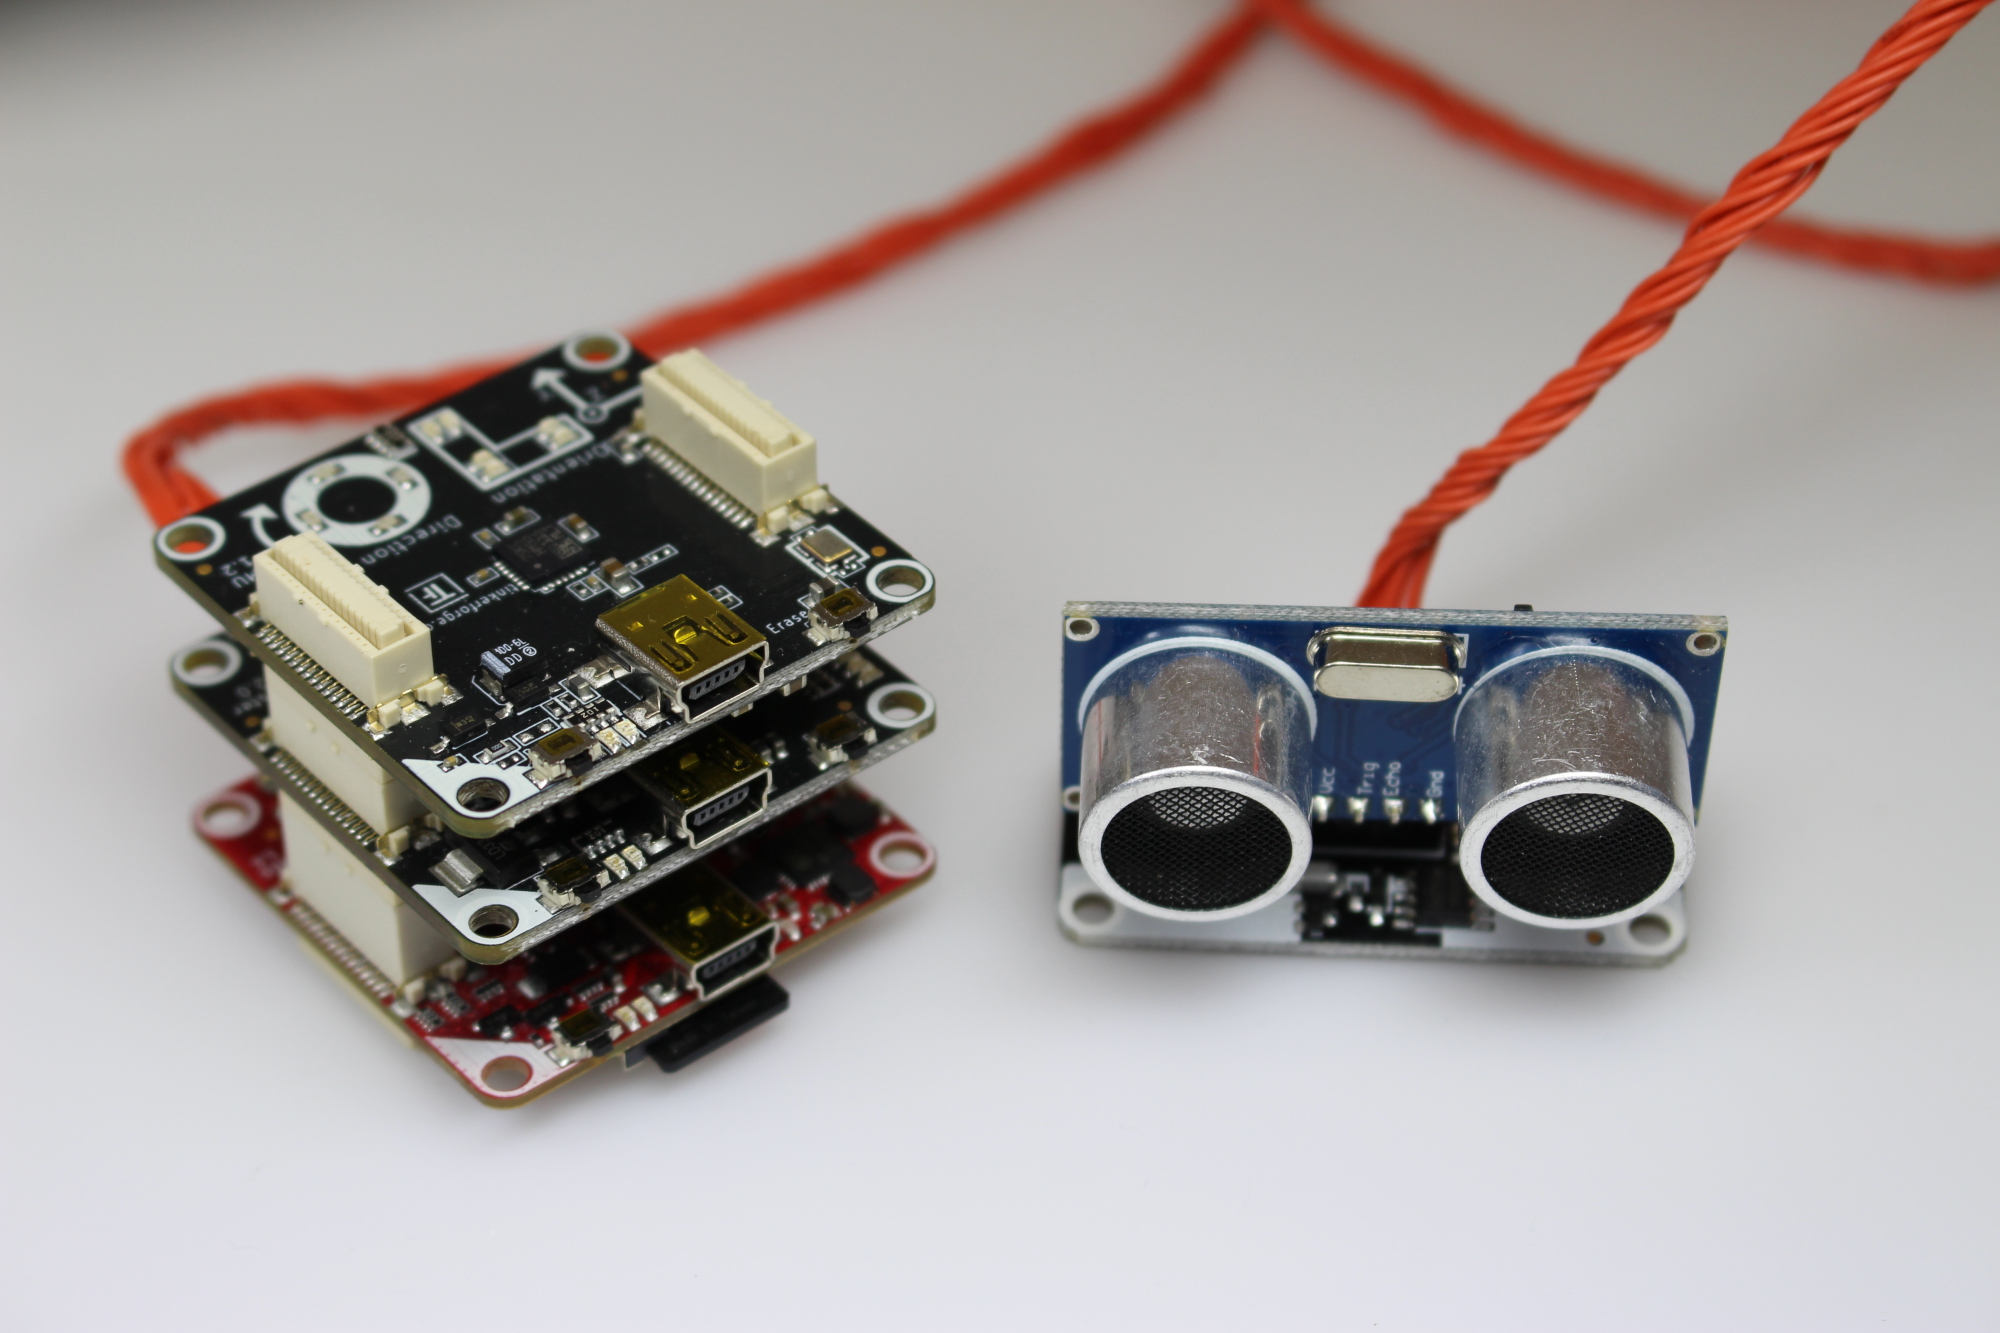
\includegraphics[width=0.5\textwidth]{fig/Tinkerforge.png}
	\caption{Beispielhaftes Tinkerforge System (Bricks mit Ultraschallmodul) (Quelle: http://www.heise.de)}
	%http://www.heise.de/imgs/18/1/3/9/9/7/1/4/IMG_0866-6a15d221db4848a1.jpeg
\end{figure}

\begin{table}[h]
\begin{tabular}{p{0.5\textwidth} | p{0.5\textwidth}}


\textbf{Vorteile} & \textbf{Nachteile} \\ \hline
	 
\begin{itemize}
\item Einfache und modulare Schnittstelle zum Boardcomputer
\item Einfach erweiterbar mit zusätzlichen Modulen (z.B Sensoren)
\item Viele benötigte Module Vorhanden: Schrittmotoren, Distanzsensoren, Liniensensoren und Farbsensoren
\end{itemize}
 &
\begin{itemize}
\item Grosser Aufwand für eigene Module(Abhängigkeit zu Tinkerforge)
\item Debugging könnte Probleme bereiten (Linuxberiebsystem) 
\end{itemize}
\end{tabular}
\end{table}


\begin{table}[h]
\begin{tabular}{p{0.5\textwidth}p{0.5\textwidth}}


\textbf{Risiken} & \\ \hline
	 
\begin{itemize}
\item Es sind nicht alle benötigten Module vorhanden oder erfüllen die Anforderungen => eventuell aufwändige Hardwareanbindung nötig
\item Die Rechenperformance reicht nicht (unwahrscheinlich)
\end{itemize}
&
\begin{itemize}
\item Teure Hauptplatine, ein Defekt könnte das Budget belasten.
\item Lieferung aus Deutschland, eventuelle lange Lieferzeit (wichtig bei Defekt)
\end{itemize}

 
\end{tabular}
\end{table}

\pagebreak

% !TEX root = morphkasten.tex

\section{Mini-Computer}


%##############
\subsection{Raspberry Pi 1}

\begin{figure}[h!]%Position festigen
\centering
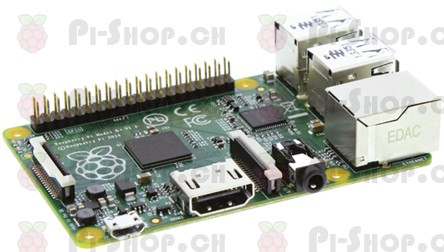
\includegraphics[width=0.5\textwidth]{fig/PI1.jpg}
\caption{Raspberry Pi 1 (Quelle: https://www.pi-shop.ch)}
\label{fig:PI1}
\end{figure}

\begin{table}[h]
\begin{tabular}{p{0.5\textwidth} | p{0.5\textwidth}}


 \textbf{Vorteile} & \textbf{Nachteile} \\ \hline
	 
\begin{itemize}
\item Zuverlässig
\item Einfache Ansteuerung
\item Kompatible Komponenten (Kamera)
\item Geläufiges Betriebssystem
\item Geringer Energieverbrauch
\end{itemize}

 
 &
 
\begin{itemize}
\item Wenig Leistung (Echtzeit)
\item Platzverbrauch auf Fahrzeug
\end{itemize}

\end{tabular}
\end{table}

\begin{table}[h]
\begin{tabular}{p{0.5\textwidth}p{0.5\textwidth}}


 \textbf{Risiken} & \\ \hline
	 
\begin{itemize}
\item Echtzeitbildverarbeitung funktioniert nicht
\item Benötigt zu viel Platz auf Fahrzeug
\end{itemize}

 
\end{tabular}
\end{table}

\pagebreak


%##############
\subsection{Raspberry Pi 2}

\begin{figure}[h!]%Position festigen
\centering
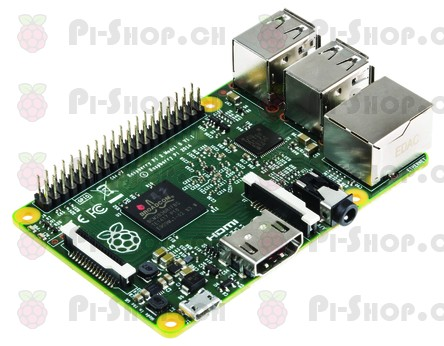
\includegraphics[width=0.5\textwidth]{fig/PI2.jpg}
\caption{Raspberry Pi 2 (Quelle: https://www.pi-shop.ch)}
\label{fig:PI2}
\end{figure}

\begin{table}[h]
\begin{tabular}{p{0.5\textwidth} | p{0.5\textwidth}}


 \textbf{Vorteile} & \textbf{Nachteile} \\ \hline
	 
\begin{itemize}
\item Hohe Leistung (Echtzeit)
\item Zuverlässig
\item Einfache Ansteuerung
\item Kompatible Komponenten (Kamera)
\item Geläufiges Betriebssystem
\item Geringer Energieverbrauch
\end{itemize}

 
 &
 
\begin{itemize}
\item Energieverbrauch zu hoch
\item Platzverbrauch auf Fahrzeug
\end{itemize}

\end{tabular}
\end{table}

\begin{table}[h]
\begin{tabular}{p{0.5\textwidth}p{0.5\textwidth}}


 \textbf{Risiken} & \\ \hline
	 
\begin{itemize}
\item Verbraucht zu viel Energie
\item Echtzeitbildverarbeitung funktioniert trotzdem nicht
\end{itemize}
&
\begin{itemize}
\item Fehlgeschlagene Parallelisierung führt zu Ineffizienz
\item Benötigt zu viel Platz auf Fahrzeug
\end{itemize}
 
\end{tabular}
\end{table}

\pagebreak

%##############
\subsection{Banana Pi}

\begin{figure}[h!]%Position festigen
\centering
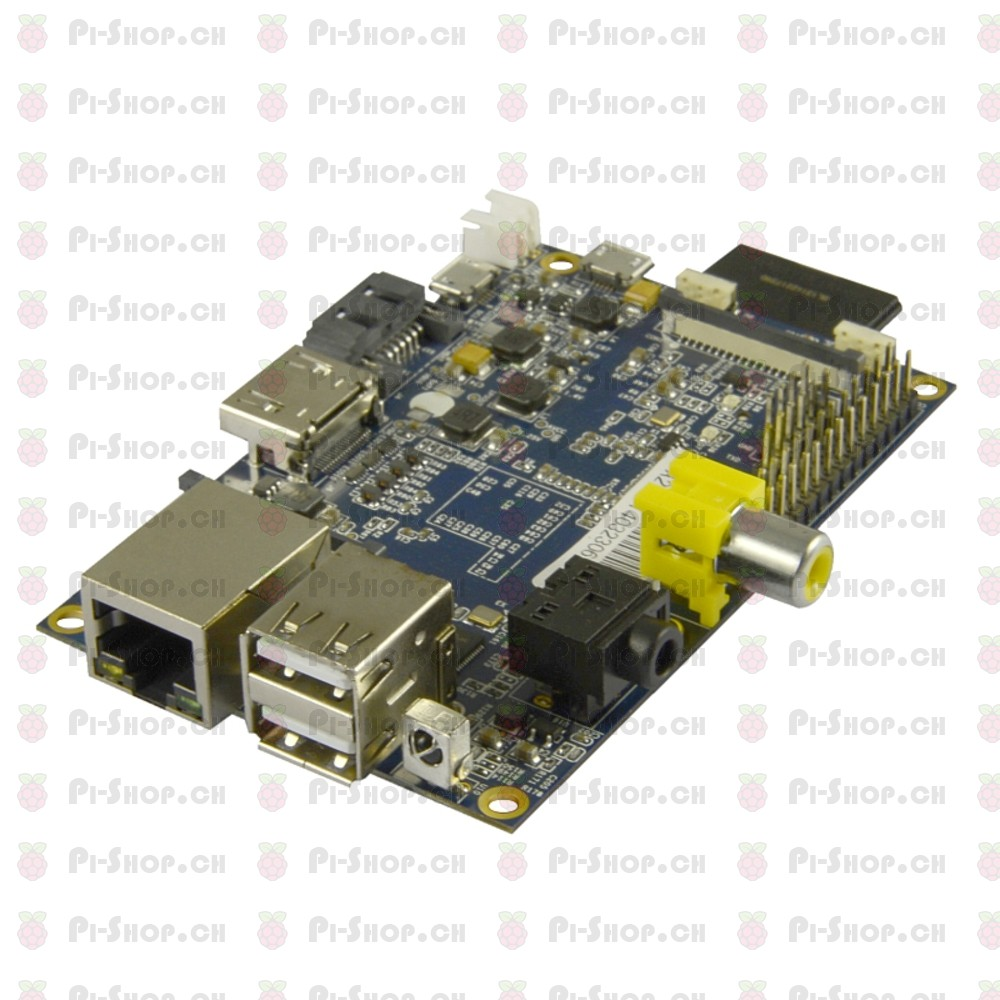
\includegraphics[width=0.5\textwidth]{fig/PIBanana.jpg}
\caption{Banana Pi (Quelle: https://www.pi-shop.ch)}
\label{fig:Banana Pi}
\end{figure}

\begin{table}[h]
\begin{tabular}{p{0.5\textwidth} | p{0.5\textwidth}}


 \textbf{Vorteile} & \textbf{Nachteile} \\ \hline
	 
\begin{itemize}
\item Minimal günstiger
\item Geläufiges Betriebssystem
\item Geringer Energieverbrauch
\end{itemize}

 
 &
 
\begin{itemize}
\item Keinerlei Erfahrung
\item Wenig Leistung (Echtzeit)
\item Platzverbrauch auf Fahrzeug
\end{itemize}

\end{tabular}
\end{table}

\begin{table}[h]
\begin{tabular}{p{0.5\textwidth}p{0.5\textwidth}}


 \textbf{Risiken} & \\ \hline
	 
\begin{itemize}
\item Zu wenig Zeit zum Einarbeiten
\item Echtzeitbildverarbeitung funktioniert nicht
\end{itemize}
&
\begin{itemize}
\item Benötigt zu viel Platz auf Fahrzeug
\end{itemize}

 
\end{tabular}
\end{table}

\pagebreak

% !TEX root = morphkasten.tex

\section{Kamera}


%##############
\subsection{Raspberry Pi Cam}

\begin{figure}[h!]%Position festigen
\centering
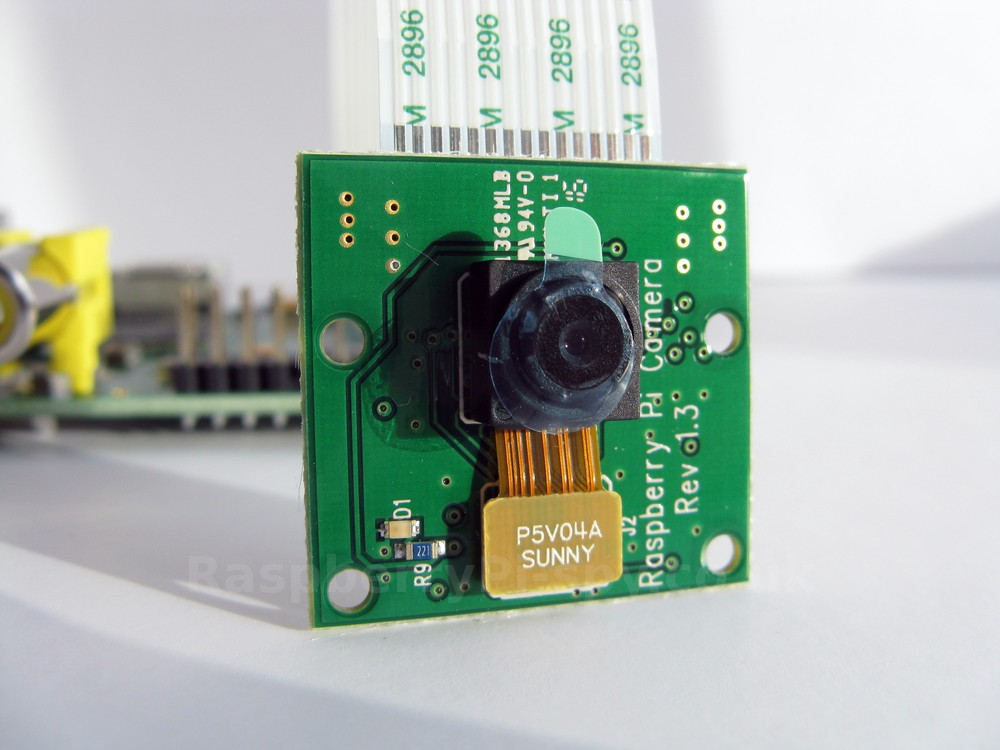
\includegraphics[width=0.5\textwidth]{fig/raspberry-pi-camera-module.jpg}
\caption{Pi Cam (Quelle: https://www.raspberrypi.org)}
\label{fig:PiCam}
\end{figure}

\begin{table}[h]
\begin{tabular}{p{0.5\textwidth} | p{0.5\textwidth}}


 \textbf{Vorteile} & \textbf{Nachteile} \\ \hline
	 
\begin{itemize}
\item Tiefe Anschaffungskosten
\item Kleine Baugrösse
\item Grosse Community
\item OpenSource Treiber
\item Gute Auflösung
\end{itemize}

 
 &
 
\begin{itemize}
\item Fester Fokus auf 1m
\item Relativ geringer Winkel mit 53.5°
\item Halterung muss erstellt werden
\item MIPI Schnittstelle erforderlich
\end{itemize}

\end{tabular}
\end{table}

\begin{table}[h]
\begin{tabular}{p{0.5\textwidth}p{0.5\textwidth}}


 \textbf{Risiken} & \\ \hline
	 
\begin{itemize}
\item Fahrbahn kann in der Kurve nicht vollständig erfasst werden
\item Objekte können nicht vollständig erfasst werden
\item Kompatibilität zu Minicomputer eingeschränkt (Nur Rasp Pi und Banana Pi)
\end{itemize}
&
\begin{itemize}
\item Kein Autofokus: Scharfstellung nicht sichergestellt
\item Farbverhalten bei unterschiedlichen Lichtverhältnissen 
\end{itemize}

 
\end{tabular}
\end{table}

\pagebreak

%##############
\subsection{Raspberry Pi Cam Noir}

\begin{figure}[h!]%Position festigen
\centering
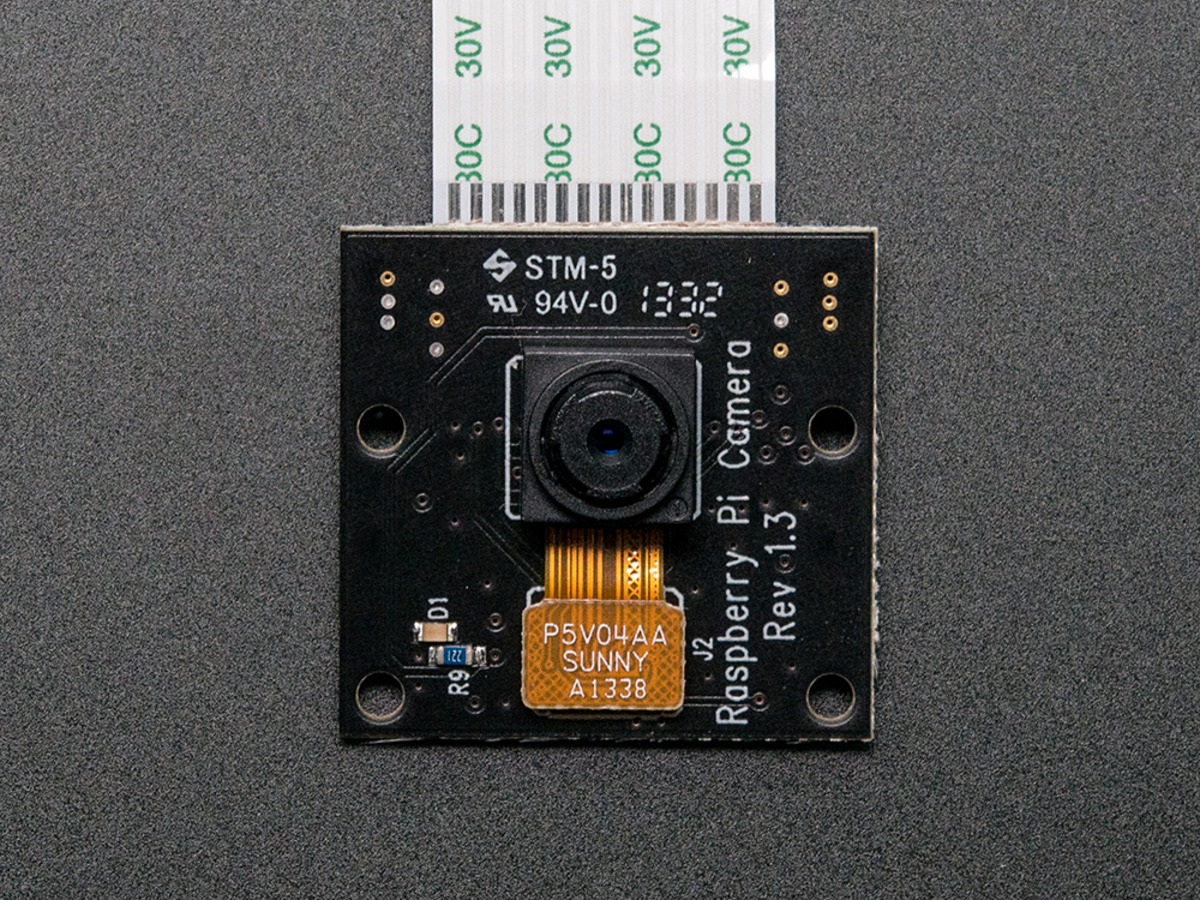
\includegraphics[width=0.5\textwidth]{fig/raspberry-pi-camera-noir.jpg}
\caption{Pi Cam Noir (Quelle: https://www.adafruit.com)}
\label{fig:PiCamNoir}
\end{figure}

\begin{table}[h]
\begin{tabular}{p{0.5\textwidth} | p{0.5\textwidth}}


 \textbf{Vorteile} & \textbf{Nachteile} \\ \hline
	 
\begin{itemize}
\item Relativ tiefe Anschaffungskosten
\item Analog Raspberry Pi Cam
\item Infrarot bei Tageslicht verwendbar, weniger empfindlich auf ändernde Lichtverhältnisse
\end{itemize}

 
 &
 
\begin{itemize}
\item Fester Fokus auf 1m
\item Relativ geringer Winkel mit 53.5°
\item Halterung muss erstellt werden
\item MIPI Schnittstelle erforderlich
\item Keine echten Farben, Erkennung derer unsicher
\end{itemize}

\end{tabular}
\end{table}

\begin{table}[h]
\begin{tabular}{p{0.5\textwidth}p{0.5\textwidth}}


 \textbf{Risiken} & \\ \hline
	 
\begin{itemize}
\item Fahrbahn kann in der Kurve nicht vollständig erfasst werden
\item Objekte können nicht vollständig erfasst werden
\item Kompatibilität zu Minicomputer eingeschränkt (Nur Rasp Pi und Banana Pi)
\end{itemize}
&
\begin{itemize}
\item Kein Autofokus: Scharfstellung nicht sichergestellt
\item Farben könnten nicht richtig erkannt werden
\item Höhere Anschaffungskosten ohne Garantie auf Erfolgsverbesserung
\end{itemize}

 
\end{tabular}
\end{table}

\pagebreak

%##############
\subsection{Webcam}

\begin{figure}[h!]%Position festigen
\centering
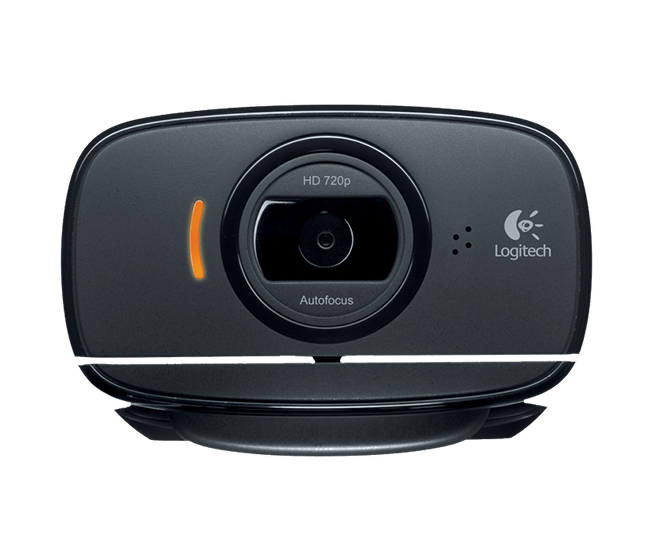
\includegraphics[width=0.5\textwidth]{fig/hd-webcam-c525-gallery.png}
\caption{Webcam (Quelle: http://www.logitech.com)}
\label{fig:Webcam}
\end{figure}

\begin{table}[h]
\begin{tabular}{p{0.5\textwidth} | p{0.5\textwidth}}


 \textbf{Vorteile} & \textbf{Nachteile} \\ \hline
	 
\begin{itemize}
\item Grosse Modellvielfalt
\item Autofokus
\item Grosser Blickwinkel mit ca 80° horizontal
\item USB-Universalschnittstelle
\item Halterung oftmals integriert
\end{itemize}

 
 &
 
\begin{itemize}
\item Höhere Anschaffungskosten
\item Kamerafunktionalitäten nur mit Herstellertreiber (proprietär)
\item Treiber meist nur für Windows erhältlich
\item Grössere Abmasse
\end{itemize}

\end{tabular}
\end{table}

\begin{table}[h]
\begin{tabular}{p{0.5\textwidth}p{0.5\textwidth}}


 \textbf{Risiken} & \\ \hline
	 
\begin{itemize}
\item Vorteile der Kamera können nicht genutzt werden
\item Kamerasystem zu gross, müsste zerlegt werden
\end{itemize}
&
\begin{itemize}
\item Hohe Kosten belasten Budget zu stark
\end{itemize}

 
\end{tabular}
\end{table}

\pagebreak

% !TEX root = ../Dokumentation.tex
\subsection{Fahrbahnerkennung}
\textbf{Funktionsbeschrieb}\\
Die Fahrbahnerkennung soll primär mittels Kamera umgesetzt werden. Dazu werden Bilder aus dem zu Verfügung gestellten Bilderpool entnommen, mit OpenCV in Graustufen umgewandelt und anschliessend einer Kantenanalyse unterzogen. Dazu wird ein eigener Algorithmus verwendet, der jeweils eine Bildzeile als Graph einer Funktion $y = f(x)$ angeschaut, wobei $x$ der Pixelkoordinate der Spalte und $y$ dem Graustufenwert des Pixels entspricht.\\
Anhand der vorhandenen Informationen kann die Fahrbahn und demzufolge während der Fahrt der Korrekturvektor ermittelt werden. Die Korrektur selber soll mittels PID-Regelung realisiert werden, um eine ruhige Fahrt zu erreichen.\\
\textbf{Komponentenbeschrieb}
\begin{figure}[h!]%Position festigen
\centering
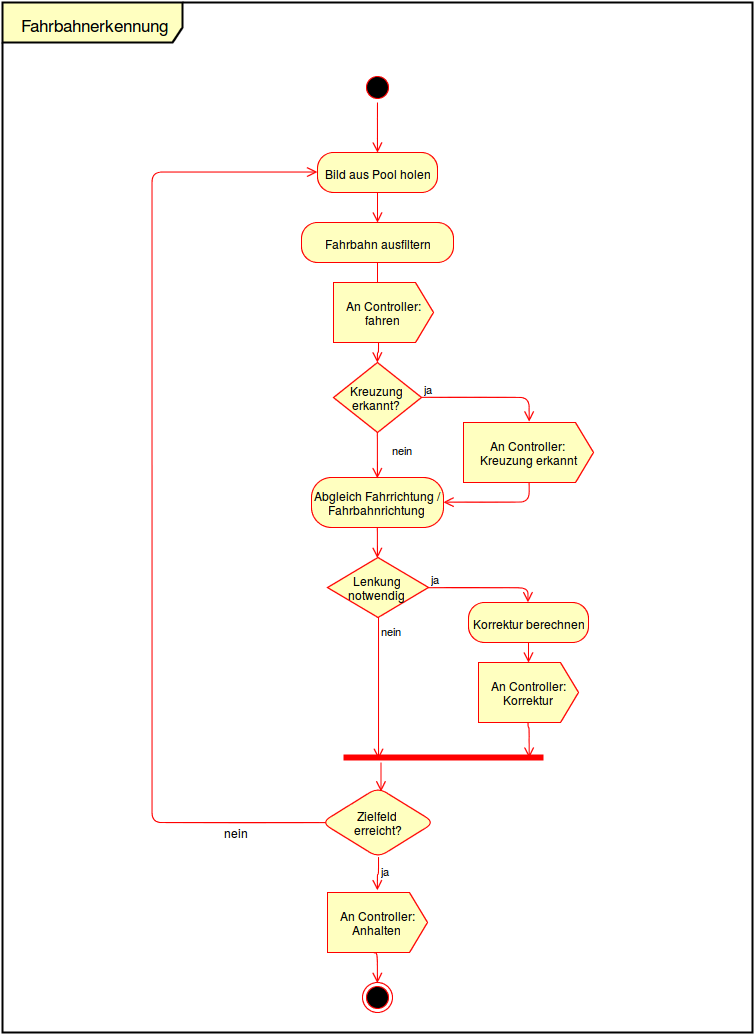
\includegraphics[width=0.6\textwidth]{03_Loesungskonzept/pictures/Fahrbahnerkennung.png}
\caption{Aktivitätendiagramm Fahrbahnerkennung}
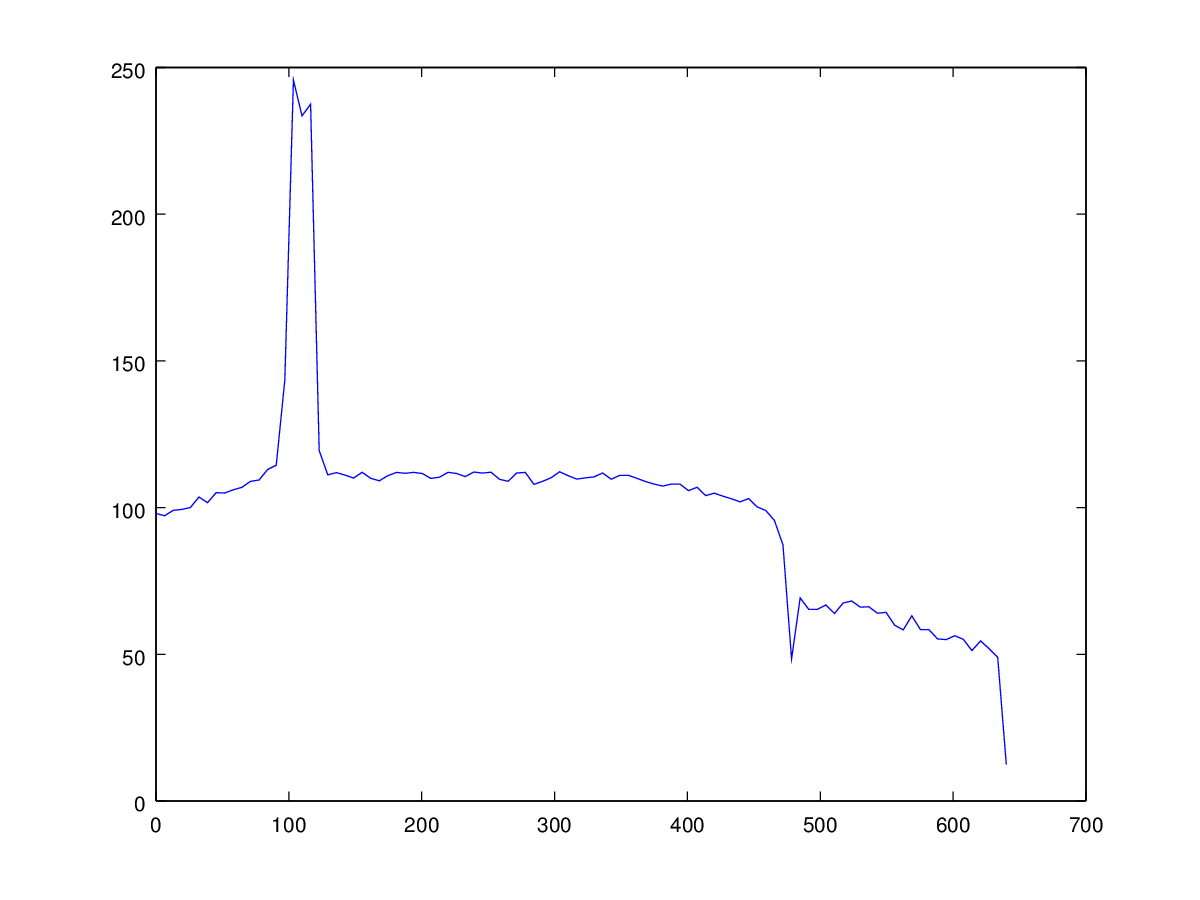
\includegraphics[width=0.6\textwidth]{03_Loesungskonzept/pictures/graphPicture.png}
\caption{Graph der Graustufenwerte einer Bildzeile}
\label{fig:grayscale}
\end{figure}\\
Die Fahrbahnerkennung wird als eigener Thread auf dem Raspberry Pi realisiert und in C++ objektorientiert umgesetzt. Für die Kantenerkennung wird jede Zeile eines Bildes als Funktion angeschaut und falls die Änderungsrate den Filterwert überschreitet eine Kante erkannt (Abbildung). \\
Im Anschluss wird im unteren Bereich des Bildes von innen nach aussen die Fahrbahn gesucht. Dazu werden jeweils in beide Richtungen die ersten Kanten gesucht, über mehrere Punkte fixiert und danach alle übrigen Kanten entfernt.\\
Da die Fahrbahn keine Sprunghaften Änderungen aufweisen kann, wird die Kantendetektierte Matrix von unten nach oben durchgesehen und alle Kanten, die in $x$ - Richtung eine zu grosse Abweichung von der erkannten Fahrbahn aufweisen entfernt, so dass nur noch die rechte und linke Fahrbahnbegrenzung übrig bleibt. Die Mitte zwischen diesen Kanten wird anschliessend in die Zielspur umgewandelt.\\
\textbf{Begründung}\\
Mit der beschriebenen Vorgehensweise kann der Aufwand pro Bild gegenüber OpenCV deutlich reduziert werden, da die Operationen ausschliesslich für die Fahrbahnerkennung erstellt werden. Die Tests haben die Realisierbarkeit dieser Vorgehensweise als machbar und fexibel aufgezeigt.\\
\textbf{Berechnungen}\\
Komplexität des Algorithmus, jedes Bild wird als eine $n\times{m}$ Matrix $M$ betrachtet wobei $n=x$ = Spaltenzahl und $m$ = Zeilenzahl. Die Resultate der Kantenerkennung werden in einer zweiten $n\times{m}$ Matrix $M_1$ gespeichert, welche für die weiteren Berechnungen verwendet wird.
\begin{itemize}
\item Iteration für Kantenerkennung:
\[
n \cdot m \leq n \cdot n \text{ wenn } n\geq m \rightarrow \mathcal{O}(n^2) \text{ mit den Zeugen }C=1 \text{ und } k = m
\]
\item Iteration für Kantenfindung Fahrbahn:
\[
10m \leq 10n  \text{ wenn } n\geq m \rightarrow \mathcal{O}(n) \text{ mit den Zeugen }C=10 \text{ und } k = m
\]
\item Iteration für Fahrbahnausfilterung und das Erzeugen der Sollspur:
\[
n \cdot m \leq n \cdot n \text{ wenn } n\geq m \rightarrow \mathcal{O}(n^2) \text{ mit den Zeugen }C=1 \text{ und } k = m
\]
\item Zusammengezogene Schätzung der Komplexität:
\begin{align*}
2(n^2) + 10n &\leq 2n^2 + 10n^2 \text{ wenn } n\geq 1\\
             &= 12n^2\\
             &\rightarrow \mathcal{O}(n^2) \text{ mit den Zeugen }C=12 \text{ und } k = m
\end{align*}
\end{itemize}
Formeln für die Berechnungen:
\begin{itemize}
\item Kantenfindung $h=$ Grenzwert für die Änderungsrate um eine Kante zu ermitteln und $y_1$ der Wert des Pixels in der Zielmatrix $M_1$:
\[
y = f(x) = \text{ Graustufen des Pixels }0 \leq y \leq 255
\]
$x:=1 \text{ to } n-2 \text{ step } 1$\\ 
$\textbf{if } f(x+2)-f(x) \geq h \textbf{ then } y_1 = 255 \textbf{ else } y_1 = 0$\\
\end{itemize}
\textbf{Testergebnisse}\\

% !TEX root = morphkasten.tex

\section{Containererkennung (grob)}


%##############
\subsection{Distanz und Farbsensor}

\begin{figure} [hbp]
	\centering
	\includegraphics[width=0.5\textwidth]{fig/Containererkennung_2.png}
	\caption{Beispielhafte Containererkennung mit Distanz- und Farbsensoren}
\end{figure}

\begin{table}[h]
\begin{tabular}{p{0.5\textwidth} | p{0.5\textwidth}}


 \textbf{Vorteile} & \textbf{Nachteile} \\ \hline
	 
\begin{itemize}
\item Präzise Erkennung des Containers (wahrscheinlich)
\item Mehrfachverwendung mit anderen Anwendungen denkbar
\item Kostengünstig
\end{itemize}

 
 &
 
\begin{itemize}
\item Unbekannte Präzision
\item Je nach Sensor Störanfälligkeit
\item Zusatzhardware(Farb und Distanzsensor) und Verkabelung nötig
\end{itemize}

\end{tabular}
\end{table}

\begin{table}[h]
\begin{tabular}{p{0.5\textwidth}p{0.5\textwidth}}


 \textbf{Risiken} & \\ \hline
	 
\begin{itemize}
\item Die Sensoren sind zu ungenau
\item Die Sensoren werden gestört
\item Das Fahrzeug kann nicht schnell genug anhalten
\end{itemize}
&
\begin{itemize}
\item Die Farbe kann auf Distanz nicht erkannt werden
\item Die Sensoren können zwischen Container und Sonstigem nicht unterscheiden
\item Die Container können bei der vollen Geschwindigkeit nicht erkannt werden
\end{itemize}

 
\end{tabular}
\end{table}

\pagebreak


%##############
\subsection{Bilderkennung}
\begin{figure}[h!]%Position festigen
\centering
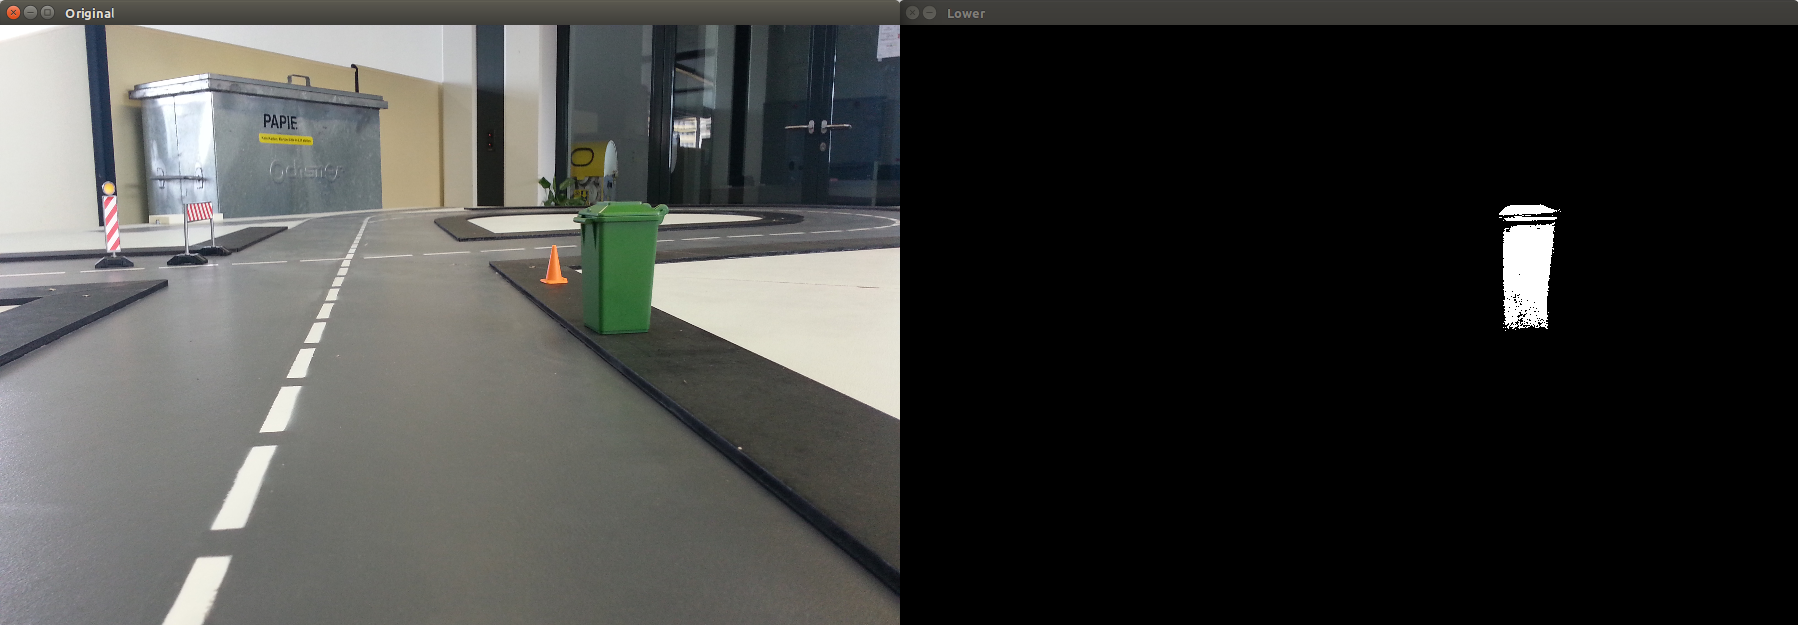
\includegraphics[width=0.7\textwidth]{fig/containererkennung_grob_bilderkennung.png}
\caption{Bilderkennung Container}
\label{fig:Bilderkennung Container}
\end{figure}

\begin{table}[h]
\begin{tabular}{p{0.5\textwidth} | p{0.5\textwidth}}


\textbf{Vorteile} & \textbf{Nachteile} \\ \hline
	 
\begin{itemize}
\item bei grösserer Distanz zu Container schon erkennbar
\item Containererkennung durch Form- und/oder Farberkennung
\end{itemize}

 
 &
 
\begin{itemize}
\item Algorithmus nötig
\item rechenintensiv
\end{itemize}

\end{tabular}
\end{table}

\begin{table}[h]
\begin{tabular}{p{0.5\textwidth}p{0.5\textwidth}}

\textbf{Risiken} & \\ \hline
	 
\begin{itemize}
\item bei verschiedene Lichtverhätlnissen variieren die Farben
\item Container kann zum Teil von anderen Gegeständen verdeckt sein
\end{itemize}

 
\end{tabular}
\end{table}

\pagebreak

% !TEX root = morphkasten.tex

\section{Containererkennung (detailliert)}


%##############
\subsection{Sensor}

Grafik

\begin{table}[h]
\begin{tabular}{p{0.5\textwidth} | p{0.5\textwidth}}


 \textbf{Vorteile} & \textbf{Nachteile} \\ \hline
	 
\begin{itemize}
\item Vorteil 1
\item Vorteil 2
\item Vorteil 3
\item ...
\end{itemize}

 
 &
 
\begin{itemize}
\item Nachteil 1
\item Nachteil 2
\item Nachteil 3
\item ...
\end{itemize}

\end{tabular}
\end{table}

\begin{table}[h]
\begin{tabular}{p{0.5\textwidth}p{0.5\textwidth}}


 \textbf{Risiken} & \\ \hline
	 
\begin{itemize}
\item Risiko 1
\item Risiko 2
\end{itemize}
&
\begin{itemize}
\item Risiko 3
\item ...
\end{itemize}

 
\end{tabular}
\end{table}

\pagebreak


%##############
\subsection{Bilderkennung}
Grafik

\begin{table}[h]
\begin{tabular}{p{0.5\textwidth} | p{0.5\textwidth}}


 \textbf{Vorteile} & \textbf{Nachteile} \\ \hline
	 
\begin{itemize}
\item Vorteil 1
\item Vorteil 2
\item Vorteil 3
\item ...
\end{itemize}

 
 &
 
\begin{itemize}
\item Nachteil 1
\item Nachteil 2
\item Nachteil 3
\item ...
\end{itemize}

\end{tabular}
\end{table}

\begin{table}[h]
\begin{tabular}{p{0.5\textwidth}p{0.5\textwidth}}


 \textbf{Risiken} & \\ \hline
	 
\begin{itemize}
\item Risiko 1
\item Risiko 2
\end{itemize}
&
\begin{itemize}
\item Risiko 3
\item ...
\end{itemize}

 
\end{tabular}
\end{table}

\pagebreak

% !TEX root = morphkasten.tex

\section{Rechtsvortritt}


%##############
\subsection{Sensor}

\begin{figure}[h]
	\centering
	\includegraphics[width=0.3\textwidth]{fig/RechtsvortrittSensor.png}
	\caption{Mögliche Rechtsvortritt Erkennung}
\end{figure}

\begin{table}[h]
\begin{tabular}{p{0.5\textwidth} | p{0.5\textwidth}}


 \textbf{Vorteile} & \textbf{Nachteile} \\ \hline
	 
\begin{itemize}
\item Relativ einfach zu Realisieren
\item Beispielanwendungen für MC Boards vorhanden 
\end{itemize}

 
 &
 
\begin{itemize}
\item Relativ enges \"Sichtfeld\"
\item Keine Unterscheidung zwischen verschiedenen Objekten möglich
\item Zusätzliche Hardware nötig
\end{itemize}

\end{tabular}
\end{table}

\begin{table}[h]
\begin{tabular}{p{0.5\textwidth}p{0.5\textwidth}}


 \textbf{Risiken} & \\ \hline
	 
\begin{itemize}
\item Container oder andere Objekte versperren die Sicht (vor der Kreuzung)
\item Schnelle Fahrzeuge werden eventuell nicht richtig erkannt
\end{itemize}


 
\end{tabular}
\end{table}

\pagebreak


%##############
\subsection{Bilderkennung}

\begin{figure}[h!]%Position festigen
\centering
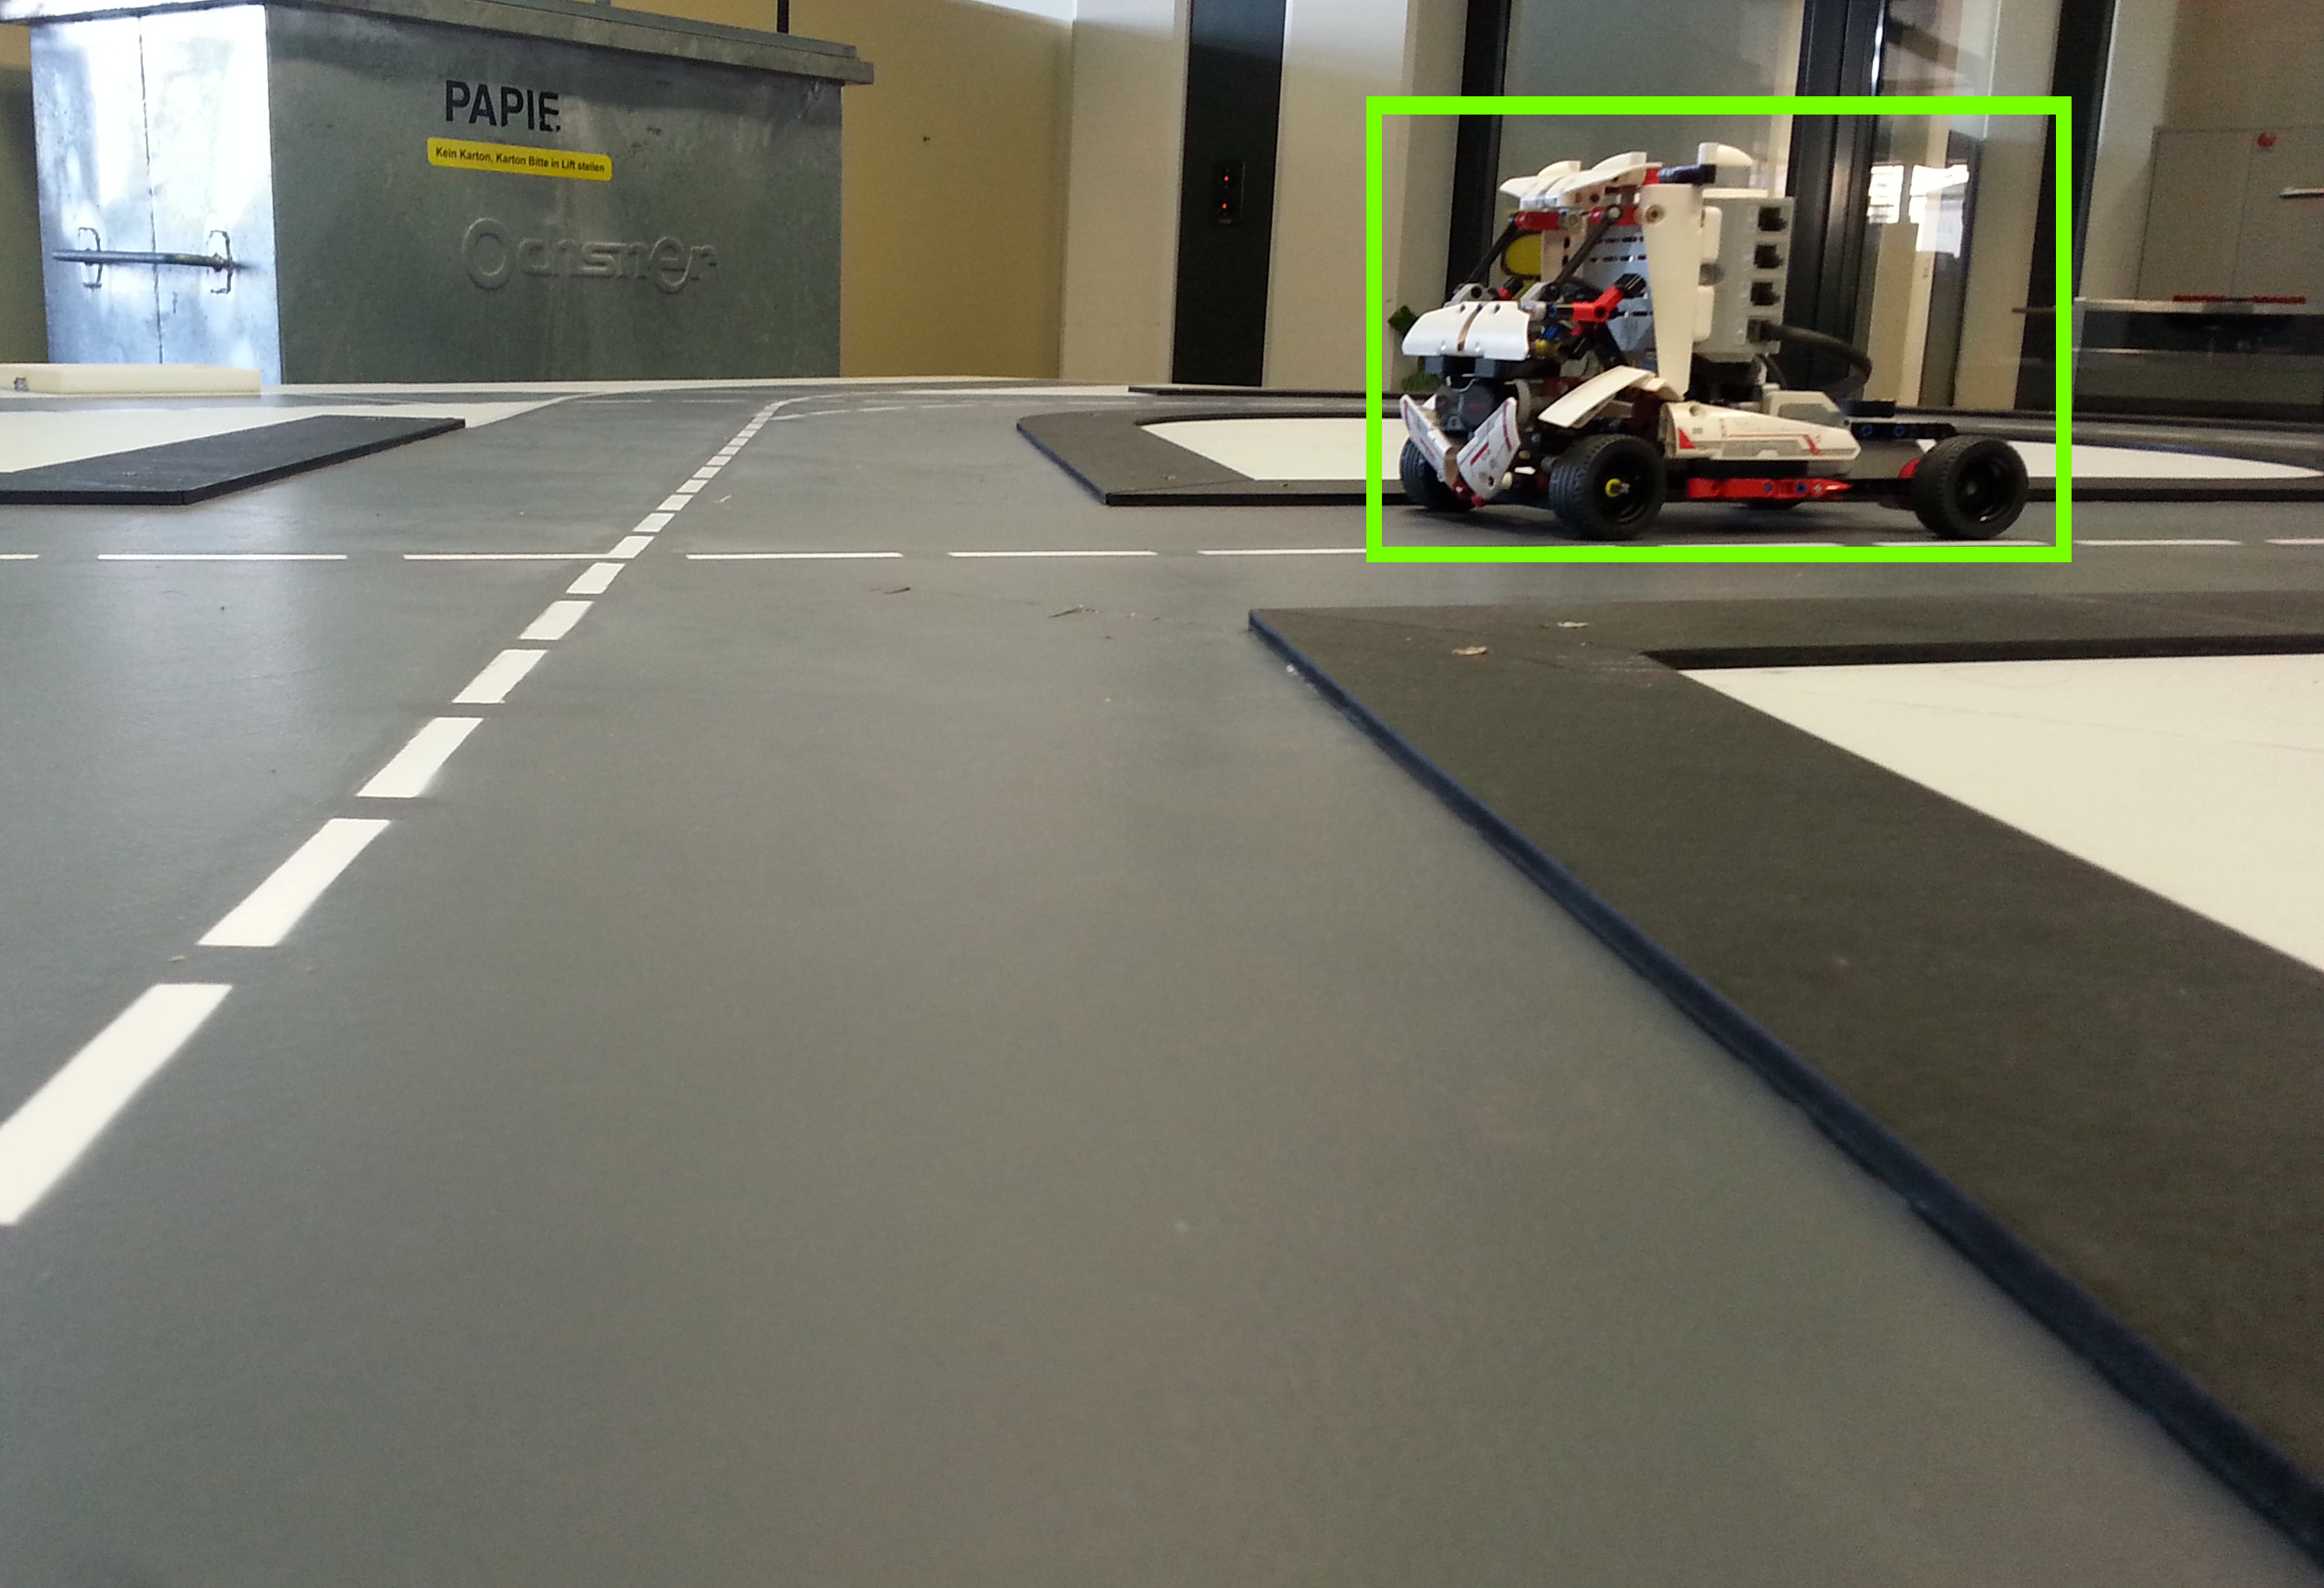
\includegraphics[width=0.7\textwidth]{fig/rechtsvortritt_bilderkennung.png}
\caption{Bilderkennung Rechtsvortritt}
\label{fig:Bilderkennung Rechtsvortritt}
\end{figure}

\begin{table}[h]
\begin{tabular}{p{0.5\textwidth} | p{0.5\textwidth}}


 \textbf{Vorteile} & \textbf{Nachteile} \\ \hline
	 
\begin{itemize}
\item Stoppen durch Vorausplnung möglich
\item Unterschiede berechnen, wie sich das andere Fahrzeug bewegt
\end{itemize}

 
 &
 
\begin{itemize}
\item Genaue Definition, was ein Fahzeug an der Kreuzung beim Rechtsvortritt ist
\item Rechenintensiv
\end{itemize}

\end{tabular}
\end{table}

\begin{table}[h]
\begin{tabular}{p{0.5\textwidth}p{0.5\textwidth}}


\textbf{Risiken} & \\ \hline
	 
\begin{itemize}
\item Fahrzeug wird auch an anderen Stellen erkannt
\item Andere Gegenstände könnten als Fahrzeug interpretiert werden

\end{itemize}

 
\end{tabular}
\end{table}

\pagebreak

% !TEX root = morphkasten.tex

\section{Programmiersprache}


%##############
\subsection{Java}

Grafik

\begin{table}[h]
\begin{tabular}{p{0.5\textwidth} | p{0.5\textwidth}}


 \textbf{Vorteile} & \textbf{Nachteile} \\ \hline
	 
\begin{itemize}
\item Vorteil 1
\item Vorteil 2
\item Vorteil 3
\item ...
\end{itemize}

 
 &
 
\begin{itemize}
\item Nachteil 1
\item Nachteil 2
\item Nachteil 3
\item ...
\end{itemize}

\end{tabular}
\end{table}

\begin{table}[h]
\begin{tabular}{p{0.5\textwidth}p{0.5\textwidth}}


 \textbf{Risiken} & \\ \hline
	 
\begin{itemize}
\item Risiko 1
\item Risiko 2
\end{itemize}
&
\begin{itemize}
\item Risiko 3
\item ...
\end{itemize}

 
\end{tabular}
\end{table}

\pagebreak


%##############
\subsection{C++}
Grafik

\begin{table}[h]
\begin{tabular}{p{0.5\textwidth} | p{0.5\textwidth}}


 \textbf{Vorteile} & \textbf{Nachteile} \\ \hline
	 
\begin{itemize}
\item Vorteil 1
\item Vorteil 2
\item Vorteil 3
\item ...
\end{itemize}

 
 &
 
\begin{itemize}
\item Nachteil 1
\item Nachteil 2
\item Nachteil 3
\item ...
\end{itemize}

\end{tabular}
\end{table}

\begin{table}[h]
\begin{tabular}{p{0.5\textwidth}p{0.5\textwidth}}


 \textbf{Risiken} & \\ \hline
	 
\begin{itemize}
\item Risiko 1
\item Risiko 2
\end{itemize}
&
\begin{itemize}
\item Risiko 3
\item ...
\end{itemize}

 
\end{tabular}
\end{table}

\pagebreak

% !TEX root = morphkasten.tex

\section{Bilderkennungs-Bibliothek}


%##############
\subsection{OpenCV}

\begin{figure}[h!]%Position festigen
\centering

\includegraphics[width=0.3\textwidth]{fig/opencv.png}
\caption{OpenCV (Quelle: https://en.wikipedia.org/wiki/OpenCV)}
\label{fig:OpenCV}
\end{figure}

\begin{table}[h]
\begin{tabular}{p{0.5\textwidth} | p{0.5\textwidth}}



 \textbf{Vorteile} & \textbf{Nachteile} \\ \hline
	 
\begin{itemize}
\item grosse Community
\item läuft auf Linux
\item ist gratis
\item kompatibel mit Java und C++
\end{itemize}

 
 &
 
\begin{itemize}
\item enthält auch viele Funktionen, welche nicht benötigt werden (komplex)
\end{itemize}

\end{tabular}
\end{table}

\begin{table}[h]
\begin{tabular}{p{0.5\textwidth}p{0.5\textwidth}}


 \textbf{Risiken} & \\ \hline
	 
\begin{itemize}
\item Ressourcenknappheit
\end{itemize}

 
\end{tabular}
\end{table}

\pagebreak


%##############
\subsection{SimpleCV}
\begin{figure}[h!]%Position festigen
\centering

\includegraphics[width=0.5\textwidth]{fig/simplecv.png}
\caption{SimpleCV (Quelle: http://google-opensource.blogspot.ch/2012\_08\_01\_archive.html)}
\label{fig:SimpleCV}
\end{figure}

\begin{table}[h]
\begin{tabular}{p{0.5\textwidth} | p{0.5\textwidth}}


 \textbf{Vorteile} & \textbf{Nachteile} \\ \hline
	 
\begin{itemize}
\item Läuft auf Linux
\item freie Software
\item kompatibel mit Java und C++
\end{itemize}

 &
 
\begin{itemize}
\item Community kleiner als bei OpenCV
\end{itemize}

\end{tabular}
\end{table}

\begin{table}[h]
\begin{tabular}{p{0.5\textwidth}p{0.5\textwidth}}


\textbf{Risiken} & \\ \hline
	 
\begin{itemize}
\item zu Problemen wird keine Lösung gefunden
\item Ressourcenknappheit
\end{itemize}
 
\end{tabular}
\end{table}

\pagebreak

% !TEX root = morphkasten.tex
\section{Anhang}
% !TEX root = morphkasten.tex


%##############
\subsection{Farbsensor}
\begin{figure}[h]
	\centering
	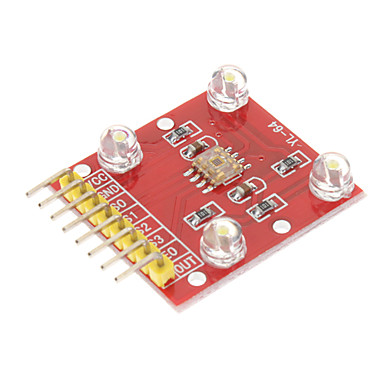
\includegraphics[width=0.5\textwidth]{fig/Farbsensor}
	\caption{Freedomboard KL25 von Freescale (Quelle: www.miniinthebox.com)}
	%http://miniimg1.rightinthebox.com/images/384x384/201310/bvlklo1383018315288.jpg
\end{figure}


\begin{table}[h]
\begin{tabular}{p{0.5\textwidth} | p{0.5\textwidth}}


 \textbf{Vorteile} & \textbf{Nachteile} \\ \hline
	 
\begin{itemize}
\item Im Preisrahmen, ein Farbsensor kostet ungefähr 10.-
\end{itemize}

 &
 
\begin{itemize}
\item Benötigt  AD Eingänge
\item Distanz abhängig
\end{itemize}

\end{tabular}
\end{table}

\begin{table}[h]
\begin{tabular}{p{0.5\textwidth}p{0.5\textwidth}}


 \textbf{Risiken} & \\ \hline
	 
\begin{itemize}
\item Distanz hat zu grossen Einfluss auf die Farberkennung
\item Die Farben lassen sich nicht zuverlässig erkennen (Sensorseite)
\end{itemize}
&
\begin{itemize}
\item Die Auswertung ist sehr aufwändig (Mikrocontrollerseitig)
\end{itemize}

 
\end{tabular}
\end{table}

\pagebreak


%##############
\subsection{Ultraschallsensoren}
\begin{figure}[h]
	\centering
	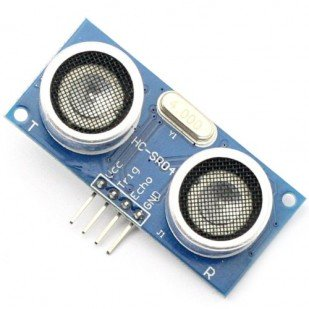
\includegraphics[width=0.5\textwidth]{fig/ultraschallsensor.png}
	\caption{Beispielhaftes Tinkerforge System (Bricks mit Ultraschallmodul) (Quelle: www.generationrobots.com)}
	%http://www.generationrobots.com/2653-large_default/ultraschallsensor-hc-sr04.jpg
\end{figure}

\begin{table}[h]
\begin{tabular}{p{0.5\textwidth} | p{0.5\textwidth}}


\textbf{Vorteile} & \textbf{Nachteile} \\ \hline
	 
\begin{itemize}
\item Erschwinglich, ein Sensor kostet ungefähr 5.Fr
\item Unempfindlich auf Störeinflüsse (Ausser andere Ultraschallsensoren)
\item Grosse Distanz (>10cm)
\end{itemize}
 &
\begin{itemize}
\item Kann nicht als als Liniensensor eingesetzt werden
\item Keine klaren Grenzen (relativ grosser Abstrahlwinkel)
\end{itemize}
\end{tabular}
\end{table}


\begin{table}[h]
\begin{tabular}{p{0.5\textwidth}p{0.5\textwidth}}


 \textbf{Risiken} & \\ \hline
	 
\begin{itemize}
\item Andere Ultraschallsensoren stören die Messung
\item Der Bereich ist zu ungenau
\end{itemize}
&
\begin{itemize}
\item Die Anbindung funktioniert nicht richtig
\end{itemize}

 
\end{tabular}
\end{table}

\pagebreak

%##############
\subsection{Infrarotsensoren}
\begin{figure}[h]
	\centering
	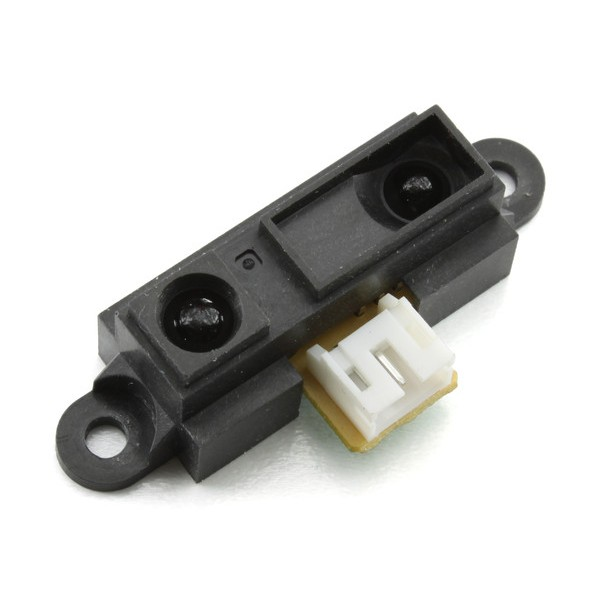
\includegraphics[width=0.5\textwidth]{fig/Infrarotsensor.jpg}
	\caption{Infrarotsensor (Quelle: www.tinkerforge.com)}
	%https://www.tinkerforge.com/de/shop/media/catalog/product/cache/2/image/600x600/9df78eab33525d08d6e5fb8d27136e95/s/e/sensor_gp2y0a21yk0f_tilted_600.jpg
\end{figure}
%http://www.farnell.com/datasheets/1725394.pdf

\begin{table}[h]
\begin{tabular}{p{0.5\textwidth} | p{0.5\textwidth}}


\textbf{Vorteile} & \textbf{Nachteile} \\ \hline
	 
\begin{itemize}
\item Kostengünstig (Sensor und Empfänger kosten zusammen 1.7Fr)
\item Kann als Liniensensor und Rad-Encoder eingesetzt werden.
\item Eher klaren Grenzen (kleiner Abstrahlwinkel)
\end{itemize}
 &
\begin{itemize}
\item Benötigt zwei AD Eingänge
\item Sind empfindlich auf UV-Licht
\item Geringe Reichweite (je nach Typ nur bis 5mm)
\item Als Liniensensor: Nicht senkrechtes Abtasten ist problematisch
\end{itemize}
\end{tabular}
\end{table}


\begin{table}[h]
\begin{tabular}{p{0.5\textwidth}p{0.5\textwidth}}


 \textbf{Risiken} & \\ \hline
	 
\begin{itemize}
\item Die Sensoren werden gestört
\item Die Sensoren sind zu ungenau
\end{itemize}
&
\begin{itemize}
\item Die Anbindung funktioniert nicht richtig
\end{itemize}

 
\end{tabular}
\end{table}

\pagebreak

\end{document}